\documentclass[a4paper,8pt,twocolumn]{article} % 改为双栏
\usepackage[UTF8]{ctex}
\usepackage{graphicx}  
\usepackage{amsmath}
\usepackage{amsthm}
\usepackage[most]{tcolorbox}
\usepackage{tikz}
\usepackage{wrapfig}  %使用图文混排的宏包
\usepackage{amssymb}
\usepackage{booktabs} % 已加载一次,此处为重复
\usepackage{float}
\usepackage{ulem}
\usepackage{url}% 超链路
\usepackage{bm}% 加粗部分公式
\usepackage{multirow} % 已加载一次,此处为重复
\usepackage{epsfig} % 通常推荐使用 graphicx 替代 epsfig
\usepackage{longtable}% 长表格 - 注意: longtable 不能直接在 twocolumn 模式下工作。

\usepackage{supertabular}% 跨页表格 - 与 longtable 在 twocolumn 模式下有类似问题。
\usepackage[utf8]{inputenc} % ctex 通常会处理好输入编码
\usepackage{algorithm}
\usepackage{changepage}% 
\usepackage{enumerate}% 短编号
\usepackage{enumitem}
\usepackage{algpseudocode}
\usepackage{caption}% 设置标题
\usepackage[AutoFallBack=true]{xeCJK}
\usepackage[style=gb7714-2015,backend=biber]{biblatex}
\addbibresource{reference.bib}%必须加后缀
\usepackage{listings} % 插入代码用到

\setCJKfallbackfamilyfont{\CJKrmdefault}{SimSun.ttf}
\lstset{
    basicstyle=\ttfamily,
    % backgroundcolor=\color{lightgray}, % 考虑移除此行,或选择一个非常非常浅的灰色
    keywordstyle=\color{blue},
    commentstyle=\color{green},
    stringstyle=\color{red},
    breaklines=true,
    captionpos=b,
    frame=single
}
\lstdefinestyle{Python}{
	language        =   Python, % 语言选Python
	basicstyle      =   \zihao{-5}\ttfamily,
	numberstyle     =   \zihao{-5}\ttfamily,
	keywordstyle    =   \color{blue},
	keywordstyle    =   [2] \color{teal},
	stringstyle     =   \color{magenta},
	commentstyle    =   \color{red}\ttfamily,
	breaklines      =   true,   % 自动换行,建议不要写太长的行
	columns         =   fixed,  % 如果不加这一句,字间距就不固定,很丑,必须加
	basewidth       =   0.5em,
}
% \usepackage{multirow} % 重复加载
\usepackage{indentfirst}% 中文首行缩进
\usepackage[left=2.50cm,right=2.50cm,top=2.80cm,bottom=2.50cm]{geometry}% 页边距设置
\renewcommand{\baselinestretch}{1.5}% 定义行间距(1.5) % 保留原始设置,但请参考上面的注释。
\usepackage{hyperref}% 输出汉字
\usepackage{afterpage}
\usepackage{abstract}% 两栏文档,一栏摘要及关键字宏包
\newcommand\myemptypage{
    \null
    \thispagestyle{empty}
    \addtocounter{page}{-1}
    \newpage
    }
\usepackage{fancyhdr} %设置全文页眉、页脚的格式
\pagestyle{fancy}

% \fancyhf{} % 清除所有页眉页脚域
% \fancyhead[L]{\kaishu · \thepage ·}
% \fancyhead[C]{\kaishu 中国安全生产科学技术} % 替换为实际期刊名称
% \fancyhead[R]{\kaishu 第 19 卷}            % 替换为实际卷号
% \renewcommand{\headrulewidth}{0.4pt}     % 页眉下的横线
% \renewcommand{\footrulewidth}{0pt}       % 页脚上没有横线 (默认)
% % 同时,为 'plain' 页面样式进行设置 (例如章节首页,如果使用 'book' 类)
% \fancypagestyle{plain}{%
%   \fancyhf{}%
%   \fancyfoot[C]{\thepage}%
%   \renewcommand{\headrulewidth}{0pt}%
% }
% 上述 fancyhdr 设置仅为建议。您需要调整文本和字体。
\usepackage{tikz}
\hypersetup{colorlinks=true,linkcolor=black}% 去除引用红框,改变颜色
\usepackage{array}
\renewcommand{\abstracttextfont}{\fangsong}% 摘要内容字体为仿宋
\renewcommand{\abstractname}{\textbf{摘\quad 要}}% 更改摘要二字的样式
\newtcolorbox{myproof}{
  colback=gray!5, % 背景颜色为浅灰色
  colframe=white, % 边框颜色为白色
  coltitle=black, % 标题颜色为黑色
  fonttitle=\bfseries, % 标题字体为加粗
  breakable, % 允许跨页
  enhanced jigsaw % 支持断行
}
\usepackage{subcaption}
% \hypersetup{colorlinks=true,linkcolor=black}% 此处重复设置
%%%%%%%%%%%%%%%%%%%%%%%%%%%%%%%%%%%%%%%%%%%%%%%%%%%%%%%%
\title{\fontsize{18pt}{27pt}\selectfont% 小四字号,1.5倍行距
	{\heiti% 黑体 
		考虑企业社会责任的应急物资协同储备:Stackelberg博弈模型
  }}% 题目
%%%%%%%%%%%%%%%%%%%%%%%%%%%%%%%%%%%%%%%%%%%%%%%%%%%%%%%%
\author{\fontsize{12pt}{18pt}\selectfont% 小四字号,1.5倍行距
	{\fangsong% 仿宋
		张珂\footnote{zhangke.bupt@hotmail.com},周吉林% 标题栏脚注
  } }
%%%%%%%%%%%%%%%%%%%%%%%%%%%%%%%%%%%%%%%%%%%%%%%%%%%%%%%%
\date{\today}% 日期(这里避免生成日期) % 如果不希望在作者下方显示日期,可以使用 \date{}
%%%%%%%%%%%%%%%%%%%%%%%%%%%%%%%%%%%%%%%%%%%%%%%%%%%%%%%%
\usetikzlibrary{arrows, shapes.geometric}
\tikzstyle{process} = [rectangle, minimum width=3cm, minimum height=1cm, text centered, draw=black]
\tikzstyle{arrow} = [thick,->,>=stealth]
\begin{document}
%制作封面
\begin{titlepage}    
\vskip 5cm
\quad
    \begin{center}
        \par
\begin{figure}[H] % 在 titlepage 中使用 [H] (来自 float 宏包) 尝试固定图片位置
		    \centering
		    
\includegraphics[width=0.8\linewidth]{basic_pictures/image.png}
		    % \label{fig:enter-label} % 封面图片的标签可能意义不大
		\end{figure}
		\vskip -1cm
	\heiti \zihao{-1} 应急物流期末大作业
		\vskip 1cm
		\par
            \centerline{
\includegraphics[width=0.30\textwidth]{basic_pictures/bupt.jpg}} %插入图片
        \par  \vskip 1cm
  \begin{table}[H] % 在 titlepage 中使用 [H]
		\centering
		\begin{LARGE}
			\begin{tabular}{p{2cm} p{10cm}<{\centering}}
			\kaishu\zihao{-2}	题 目: &  \kaishu\zihao{-2}  考虑企业社会责任的应急物资协同储备:Stackelberg博弈模型\\ \cline{2-2}
			\end{tabular}
		\end{LARGE}		
	\end{table}
	\begin{table}[H] % 在 titlepage 中使用 [H]
		\centering
		\begin{Large}
			\begin{tabular}{p{3cm} p{7cm}<{\centering}}
		\kaishu\zihao{-3}		姓 \qquad 名: & \kaishu\zihao{-3} 张珂 \quad  周吉林  \\ \cline{2-2}
        \kaishu\zihao{-3}		学 \qquad 号: &  \zihao{-3} 2021211748 2022212202\\ \cline{2-2}
		\kaishu\zihao{-3}		学 \qquad 院:      & \kaishu\zihao{-3} 智能工程与自动化学院   \\ \cline{2-2}
		\kaishu\zihao{-3}		专 \qquad 业:      & \kaishu\zihao{-3} 邮政工程   \\ \cline{2-2}
        \kaishu\zihao{-3}		选 \qquad 题:      & \kaishu\zihao{-3} 选题二  \\ \cline{2-2}
			\end{tabular}
		\end{Large}		
	\end{table}
 \vskip 1cm
{\songti\zihao{3} \today}  
\end{center}
\end{titlepage}
% 使主论文的标题、作者、摘要跨栏显示
\twocolumn[
  \begin{@twocolumnfalse} % 确保 \twocolumn[...] 内的内容按单栏排版
    \maketitle % 生成标题、作者、日期
    \thispagestyle{fancy} % 对包含标题的当前页应用 fancy 页面样式
    \begin{abstract}
    \noindent % 摘要通常不首行缩进
    为应对突发灾害事件,构建高效的应急物资储备体系至关重要。本研究聚焦于政府与企业在应急物资储备中的多主体协同问题,构建了一个基于Stackelberg博弈的政企协同储备决策模型。该模型将政府作为领导者,企业作为跟随者,综合考虑了政府实物储备、企业实物储备、考虑企业社会责任的企业捐赠以及企业生产能力储备四种储备方式。针对应急物资需求的随机性,本研究基于历史灾害数据拟合了反高斯分布作为需求概率模型,并与传统的均匀分布进行了对比分析。通过序列最小二乘二次规划算法对模型进行求解,获得了不同情景下的最优储备决策。研究结果表明:应急物资需求分布形态对最优储备结构具有显著影响,反高斯分布下模型更倾向于依赖灾后生产能力;企业社会责任的激励效应对企业捐赠量有积极作用;灾害发生概率、各项成本参数(如存储成本、采购成本、代储成本)、补贴水平及市场价格等因素均对政府和企业的最优储备策略产生不同程度的影响。本研究为制定更贴合实际、更具经济效益的应急物资协同储备契约和激励机制提供了理论依据与决策参考。    
    \par\vspace{1ex} % 关键词前增加少量垂直间距
    \noindent\textbf{关键词:} 应急物资;协同储备;Stackelberg博弈;契约设计;企业社会责任
    \end{abstract}
    \vspace{2em} % 摘要后增加一些空间,再开始双栏正文
  \end{@twocolumnfalse}
]



\section{背景介绍}

我国领土辽阔、地形复杂,地震、干旱、风雹、洪涝等自然灾害频发,对人民生命财产安全构成严重威胁。据统计,2023年各类自然灾害共造成9544.4万人次受灾,倒塌损坏房屋227.3万间,直接经济损失高达3454.5亿元 \cite{MEM2024disaster}。突发性灾害事件应急处置需要在短时间内做出反应,这需要大量的救援设备、食物、医药用品等各类应急物资 \cite{chen2009modern},对物流运作和需求管理提出了严峻挑战 \cite{sheu2010dynamic, chang2007scenario}。为快速响应灾情,截至2023年,我国已建成126个中央应急物资储备库,储备各类物资955万件 \cite{MEM2023floodconference}。然而,传统的单纯依靠政府采购和储备的模式面临物资单一、储存成本高昂、缺乏灵活性以及管理与调拨实施效率不高等问题 \cite{chen2014突发事件灾前应急物资政企联合储备模式, wang2023防汛物资}。因此,近年来我国积极倡导应急物流社会化 \cite{lu2009应急物资储备的社会化研究},\textbf{《“十四五”国家应急体系规划》\cite{ndrc2022}和 《国家防灾减灾救灾委员会办公室关于进一步加强应急抢险救灾物资保障体系和能力建设的指导意见》\cite{sfdrrmc2024}明确提出,要构建中央与地方分级负责、政府与社会力量协同、实物储备与产能储备相结合的现代化应急物资储备模式,鼓励引导企业参与储备,逐步推广协议储备、依托企业代储、生产能力储备等多种方式,以提升整体应急保障能力。}

为实现政企联合储备的有效协调,学者们广泛运用博弈论工具分析参与方的策略互动与最优决策。例如,\parencite{Li2022Stackelberg} 基于Stackelberg博弈框架构建了政企合作储备决策模型,分析了不同需求分布下政府与企业的最优储备量。而 \parencite{Zhang2022Evolutionary} 则从更宏观的视角出发,将社会力量纳入考量,构建了包含政府、企业和社会的应急物资联合储备三方演化博弈模型。针对非常规突发事件下的协同问题,\parencite{shao2023非常规突发事件} 构建了政企协同演化博弈模型,通过仿真分析发现适当的经济激励够显著提高物资储备效率并降低协同成本,为政府制定有效的激励政策提供了依据。此外,国际上也有研究关注通过更广泛的机制来激励和协调企业参与应急物资储备,以期达到政府和企业的双赢 \cite{egan2010private, balcik2010coordination, vanwyk2011modeling, coskun2019relief}。\parencite{vanwyk2011modeling} 针对灾害救援中需求和供应的高度不确定性,开发了优化库存成本的模型。\parencite{coskun2019relief} 则研究了双边机构合作下的救援物资库存决策问题,考虑了代理关系对决策的影响。这些博弈论和协调机制的研究为理解政企联合储备中各方的复杂互动提供了重要的理论基础,并为设计有效的激励与协调策略提供了参考。

契约机制设计是实现有效政企联合储备的另一重要研究方向,多种契约形式被引入以协调各方利益并分担风险。期权契约因其能够赋予政府在灾后面临不确定需求时延迟决策的灵活性,从而降低决策风险而受到广泛关注 \cite{rabbani2015option, wang2015prepurchasing}。\parencite{rabbani2015option} 探讨了期权契约在应急供应链中的具体应用场景和模式。\parencite{Pang2020PhysicalOption} 专门研究了实物期权契约在政企联合储备中的应用,构建了相应的模型,并详细分析了合作的可行性条件以及储备成本、期权费等因素对决策的影响。数量柔性契约作为另一种重要的协调工具,允许在预定数量上有一定的调整空间,也得到了深入研究。\parencite{nikkhoo2018coordination} 的研究表明,在人道主义物流背景下,基于数量柔性契约的救援物资采购协调有助于减少灾害损失并提高受灾群众的满意度。\parencite{chai2021考虑储备周期} 针对具有保质期的应急物资,构建了考虑储备周期的柔性采购模型,探讨了有效期约束下的最优采购策略。针对多个企业参与储备或供应的复杂情况,学者们设计了更为精巧的契约机制。例如,\parencite{Chen2023Contract} 在政府与两个代储企业合作的背景下,比较研究了简单的储备成本分担契约和包含收益分成的双边成本分担契约,并运用Stackelberg博弈推导了不同契约下的最优决策。\parencite{Li2024CooperationStrategies} 同样关注政府与两个成本或能力异质性的供应商间的合作,也对比分析了不同契约,但采用了微分博弈的方法来分析动态合作策略。期权契约的一般理论\cite{black1973pricing, barnes2002coordination,xu2010managing},也为应急储备契约的设计提供了重要的理论借鉴。这些研究表明,根据具体场景精心设计的契约能够有效协调政企合作,提升应急物资储备和供应的整体效率,并为实现各参与方的利益平衡和风险分担提供了多样化的解决方案。

为提升模型的现实解释力,部分研究将其他关键因素和更复杂的供应链结构纳入考量,使得研究更加贴近应急管理的实际需求。例如,\parencite{Gong2024Quantity} 将研究视角拓展至三级供应链,构建了由政府、制造商和原材料供应商构成的政企三方联合储备模型,在数量柔性契约下分析了各自的最优储备量,并探讨了整个供应链的协同优势。\parencite{torabi2018integrated} 关注人道主义供应链的整体优化,整合了救援物资的预置和采购规划问题,提出了综合性的决策框架。\parencite{Zheng2023CSR} 将企业的社会责任融入政企联合储备模型,探讨了企业的利他行为对物资储备量及各参与方收益的影响,为政府如何引导和激励企业履行社会责任以支持应急储备提供了新的视角。\parencite{wang2023考虑维护水平} 则关注到应急物资在储备过程中的物理损耗问题,分析了维护水平对物资完好率的影响,并将其纳入政企联合储备决策模型中,使得决策更加精细化。除了实物储备,生产能力储备作为一种重要的补充形式也受到了学者们的关注,其核心思想是在灾前储备企业的生产能力而非实物。\parencite{hu2018考虑企业生产能力} 的研究证实,通过与企业签订协议来储备其生产能力,可以在灾后快速启动生产,从而有效减少所需的实物储备量,降低库存持有成本和供应不足的风险。\parencite{zhang2016emergency} 的研究也表明,将实物储备与产能储备相结合,有助于提高政府应急资金的使用效率,减轻财政压力。\parencite{jiang2024基于代储模式} 则进一步深化了多级供应链的研究,构建了政府与制造商签订物资期权契约、制造商与关键供应商签订原材料代储契约的三级供应链模型,并探讨了这种基于代储模式的多级储备决策的适用范围和协调机制。这些研究通过引入多方参与者、不同契约形式、企业社会责任、物资维护、产能储备以及更复杂的多级供应链结构等因素,极大地丰富了政企联合储备模式的研究内容。

然而,即便多主体协同契约设计问题已经得到广泛的研究,现有研究仍存在一些问题:
\begin{itemize}
    \item \textbf{首先,关于企业社会责任的考量存在明显不足。}多数研究将企业视为纯粹逐利的经济实体\cite{Li2022Stackelberg,Chen2023Contract},而忽视了企业在应急管理中的社会责任维度。实际上,企业在应急物资储备中往往表现出显著的利他行为和社会责任意识\cite{Zheng2023CSR},这种非经济动机对储备决策的影响需要进一步的分析。
    \item \textbf{其次,现有研究对应急物资需求分布的假设过于简化。}大量文献采用均匀分布假设\cite{chai2021考虑储备周期,chen2014突发事件灾前应急物资政企联合储备模式},这与真实灾害场景下的需求特征存在显著差异,可能造成可能的决策失误。
    \item \textbf{第三,对企业多样化储备方式的协同机制研究不足。}大部分文献都是单独研究物资储备\cite{Li2022Stackelberg, li2022政企联合储备,Chen2023Contract}, 或者研究产能储备\cite{Gong2024Quantity}。将企业捐赠作为第三种储备方式,并与上述两种方式形成协同效应的研究仍属空白。
\end{itemize}

鉴于现有研究在企业社会责任考量、需求分布假设以及多样化储备方式协同等方面的不足,本研究致力于构建一个更为全面且贴近现实的政企联合应急物资储备决策模型。后续章节安排如下:在第二部分,详细阐述本文所构建模型的相应假设和符号定义,并建立政府和企业的期望收益函数。在第三部分,对模型的求解进行深入探讨,尝试证明最优决策的存在性及其数学性质。鉴于模型复杂性导致最优决策无法获得显式表达式,本研究提出采用序列二次规划求解模型,并给出具体的流程。第五部分将通过数值实验验证模型的有效性,分析关键参数对最优决策的影响,并提出相应的管理启示;最后在第六部分总结全文的主要结论,并指出未来可能的研究方向。

\section{考虑企业责任的政企联合储备决策模型}

应急物资协同储备问题涉及政府、企业2个主体,包括政府实物储备、企业实物储备、企业捐赠、企业生产能力储备4种储备方式。多主体协同应急物资储备计划的示意如图 1 所示。政府是合作主导方,企业是从属方,整个过程属于 Stackelberg 博弈\cite{Li2022Stackelberg}。

\begin{itemize}
    \item \textbf{政府实物储备} \quad 在灾害发生前,政府先提前以零售单价 $p_1$ 向市场采购 $Q$ 单位的应急物资,并以单位物资储存成本 $c_1 $储存在政府的储备库中。
    \item \textbf{企业实物储备} \quad 在灾害发生前,政府以单价 $p_2$ 提前向同盟企业采购 $q$ 单位的应急物资并交由企业进行储备。其中,企业单位物资储备成本为 $c_2$。灾害发生后,如果政府实物储备物资不足侧使用企业实物储备物资,企业的单位物资使用补助为 $s$。
    \item \textbf{企业捐赠} \quad 灾难发生后,企业捐赠$Q_j$量的物资给政府供应急使用,企业以单位物资生产成本 $e$ 参与物资的紧急生产。此次捐赠会使得企业应急物资利润增加$\lambda(m-e)\sqrt{Q_jm}$。
    \item  \textbf{企业生产能力储备} \quad 灾害发生后,在政府实物储备物资,企业实物储备以及企业捐赠的物资都使用完的前提下,企业以单位物资生产成本 $e$ 参与物资的紧急生产,并以市场单价 $m$ 卖给政府。
\end{itemize}


\subsection{前提和假设}
为保证政企协同储备模型的可实施性,做出如下一般性假设:
\begin{enumerate}
    \item 政府根据保障能力的顺序进行应急物资的使用与调配。使用顺序为政府实物储备物资、企业实物储备物资、企业生产能力储备物资。
    \item 假设物资储备周期小于保质期。1个储备周期结束后,对未使用的物资按照残值 $v$ 进行轮换。
    \item 政府选择与企业进行协同储备的前提是政府实物储备成本大于企业实物储备代储收入,满足灾害前物资单价 $p_1$ 与政府单位物资储存成本 $c_1$ 之和大于单位物资残值 $v$ 与企业单位物资代储收入 $p_2$ 之和,即满足 $p_1 + c_1 - v - p_2 > 0$。
    \item 为了促使企业积极进行实物储备与生产能力储备,单位物资使用补贴 $s$ 需要大于残值 $v$,即满足 $s > v$。同时,灾害后物资市场单价 $m$ 应大于单位物资使用补贴 $s$ 与企业单位物资代储收入 $p_2$ 之和,即满足 $m > s + p_2$。
\end{enumerate}

\subsection{应急物资需求概率分布函数}
\begin{table*}[t] % 使用 table* 环境使其跨越两列
  \centering
  \small
  \caption{政府期望收益函数}
  \label{tab:government_expected_revenue}
  % 调整列宽以适应跨页布局
  \begin{tabular}{p{4cm} p{10.5cm} } % 增加第二列的宽度
    \toprule
    灾害情况 & 政府的期望收益函数 \\
    \midrule
    灾害未发生 ($1-\alpha$) & $v Q - (p_1+c_1)Q - p_2q$  \\
    灾害发生 $\alpha$ &
    $\begin{cases}
    v(Q-x) - (p_1+c_1)Q - p_2q & 0 < x \leq Q \\
    -(p_1+c_1)Q - p_2q - s(x-Q) & Q < x \leq Q+q \\
    -(p_1+c_1)Q - p_2q - sq & Q+q < x \leq Q+q+Q_j \\
    -(p_1+c_1)Q - p_2q - sq - m(x-Q-q-Q_j) & Q+q+Q_j < x \leq U
    \end{cases}$
     \\
    \bottomrule
  \end{tabular}
\end{table*}
令概率分布函数为$F(x)$,对于均匀分布,其概率分布函数如式(1)所示:
\begin{equation} \label{eq:uniform_cdf}
F(x) = \begin{cases}
0 & x < 0 \\
\frac{x}{U} & 0 \leq x \leq U \\
1 & x > U
\end{cases}
\end{equation}
式中,$F(x)$ 为物资的需求概率分布函数;$x$ 为物资的需求量;$U$ 为最大物资需求量。这个分布是众多研究最常用的一个\cite{chai2021考虑储备周期,chen2014突发事件灾前应急物资政企联合储备模式,hu2018考虑企业生产能力}。然而这个函数可能与实际有所差别,进而导致误导性的结果 。在算例分析,我们使用概率分布拟合对概率分布进行估计。

\subsection{模型构建}
在物资储备期间灾害未发生,所有储备物资均失效。在物资储备期间灾害发生时,有以下 4 种情况:
\begin{enumerate}
    \item[1)] 当物资需求量 $0 < x \leq Q$ 时,仅使用政府实物储备物资;
    \item[2)] 当物资需求量 $Q < x \leq Q + q$ 时,所使用的储备物资为政府实物储备、企业实物储备;
    \item[3)] 当物资需求量 $Q + q < x \leq Q + q + Q_j$ 时,调用政府实物储备、企业实物储备和企业捐赠物资;
    \item[4)] 当物资需求量 $x > Q + q + Q_j$ 时,调用所有储备物资(政府实物、企业实物、企业捐赠),并启动企业生产能力满足剩余需求。
\end{enumerate}

\subsubsection{政府方期望收益}
根据上述不同情形,将政府的期望收益函数总结于表 \ref{tab:government_expected_revenue}。
灾害未发生时,所有储备物资均失效,政府利润表达式如式\ref{eq:profit_no_disaster}所示:
\begin{equation} \label{eq:profit_no_disaster}
\pi_{e,0}(Q,q) = v Q - (p_1 + c_1) Q - p_2 q
\end{equation}
式中,$\pi_{e,0}(Q,q)$ 为灾害未发生时的政府利润,元;$v$ 为单位物资残值,元;$Q$ 为政府实物储备量,件;$q$ 为企业实物储备量,件;$p_1$ 为灾害前物资单价,元;$c_1$ 为政府单位物资储存成本,元;$p_2$ 为企业单位物资代储收入,元。

灾害发生时,综合考虑 3 种收益情况,政府利润表达式如式(\ref{eq:profit_with_disaster})所示:
\begin{small}
\begin{align} \label{eq:profit_with_disaster}
\pi_{g,\alpha}(Q,q) = & \int_0^Q [v(Q-x) - (p_1+c_1)Q - p_2q] f(x)dx \notag \\
+ & \int_Q^{Q+q} [-(p_1+c_1)Q - p_2q - s(x-Q)] f(x)dx \notag \\
+ & \int_{Q+q}^{Q+q+Q_j} [-(p_1+c_1)Q - p_2q - sq] f(x)dx \notag \\
+ & \int_{Q+q+Q_j}^U [-(p_1+c_1)Q - p_2q - sq \notag \\
- & m(x-Q-q-Q_j)] f(x)dx
\end{align}
\end{small}
式中,$\pi_{e,\alpha}(Q,q)$ 为灾害发生时的政府利润,元;$x$ 为物资的需求量,件;$f(x)$ 为应急物资的概率密度函数;$s$ 为企业单位物资使用补贴,元;$m$ 为灾害后物资市场单价,元;$U$ 为最大物资需求量,件。

由式(\ref{eq:profit_no_disaster}) $\sim$ (\ref{eq:profit_with_disaster}) 可得,灾害发生概率为 $\alpha$ 时的政府利润表达式如式(\ref{eq:expected_profit})所示:
\begin{small}
\begin{align} \label{eq:expected_profit}
\pi_g(Q,q) = & (1-\alpha) \pi_{g,0}(Q,q) + \alpha \pi_{g,\alpha}(Q,q, Q_j) \notag \\
= & (1-\alpha) [v Q - (p_1+c_1)Q - p_2q] \notag \\
+ & \alpha \left\{ \int_0^Q [v(Q-x) - (p_1+c_1)Q - p_2q] f(x)dx \right. \notag \\
+ & \int_Q^{Q+q} [-(p_1+c_1)Q - p_2q - s(x-Q)] f(x)dx \notag \\
+ & \int_{Q+q}^{Q+q+Q_j} [-(p_1+c_1)Q - p_2q - sq] f(x)dx \notag \\
+ & \int_{Q+q+Q_j}^U [-(p_1+c_1)Q - p_2q - sq \notag \\
- & m(x-Q-q-Q_j)] f(x)dx \Biggr\}
\end{align}
\end{small}
式中,$\pi_e(Q,q)$ 为灾害发生概率为 $\alpha$ 时的政府利润,元;$\alpha$ 为灾害发生概率。
\subsubsection{企业期望收益}
企业在协同储备体系中的利润构成包含物资轮换残值、代储收入、应急生产收益与成本支出四个核心要素。根据储备物资调用阶段差异,企业利润函数呈现分段特征。当灾害未发生时,企业实物储备物资全部轮换获得残值收入;当灾害发生时,根据物资需求量的不同区间,企业将获得差异化收益补偿。

灾害未发生情形下,企业利润表达式如式(\ref{eq:enterprise_profit_no_disaster})所示:
\begin{equation} \label{eq:enterprise_profit_no_disaster}
{\pi}_{r,0}(q) = (v + p_2 - c_2)q
\end{equation}
式中,$\pi_{r,0}(q)$为灾害未发生时企业利润,元;$c_2$为企业单位物资储存成本,元。

灾害发生情形下,根据物资需求量 $x$ 以及政府物资调用顺序(政府实物储备 $Q$ $\rightarrow$ 企业实物储备 $q$ $\rightarrow$ 企业捐赠 $Q_j$ $\rightarrow$ 企业产能储备),企业利润函数需考虑四个物资调用阶段:
\begin{enumerate}
\item 当物资需求量 $0 < x \leq Q$ 时,仅调用政府实物储备。企业自身储备的 $q$ 全部获得残值 $v$。
\begin{equation} \label{eq:enterprise_profit_r1_mod}
\pi_{r,1}(q) = (v + p_2 - c_2)q
\end{equation}
\item 当物资需求量 $Q < x \leq Q+q$ 时,政府实物储备耗尽,开始调用企业实物储备。其中 $(x-Q)$ 部分的企业储备被使用并获得补贴 $s$,剩余的 $(Q+q-x)$ 部分获得残值 $v$。
\begin{equation} \label{eq:enterprise_profit_r2_mod}
\pi_{r,2}(q) = s(x-Q) + v(Q + q - x) + (p_2 - c_2)q
\end{equation}
\item 当物资需求量 $Q+q < x \leq Q+q+Q_j$ 时,政府实物储备和企业实物储备均耗尽。企业全部实物储备 $q$ 均获得补贴 $s$。此时,企业履行捐赠责任,捐赠 $Q_j$ 单位物资,此行为带来的净利润贡献为 $\lambda(m-e)\sqrt{Q_jm} - eQ_j$。
\begin{align} \label{eq:enterprise_profit_r3_mod}
\pi_{r,3}(q, Q_j)& = sq + (p_2 - c_2)q +\\ 
& \lambda(m-e)\sqrt{Q_jm}  \notag  - eQ_j
\end{align}
\item 当物资需求量 $x > Q+q+Q_j$ 时,政府实物储备、企业实物储备以及企业捐赠的物资均已使用完毕。企业启动生产能力储备,为超出部分 $(x-Q-q-Q_j)$ 进行紧急生产,并以单价 $m$ 售予政府,获得生产利润 $(m-e)(x-Q-q-Q_j)$。同时,企业仍获得其全部实物储备 $q$ 的补贴 $s$ 以及捐赠带来的净利润贡献。
\begin{align}
     \label{eq:enterprise_profit_r4_mod}
\pi_{r,4}(q, Q_j)& = sq + (p_2 - c_2)q +  \lambda(m-e)\sqrt{Q_jm}\notag \\ 
&- eQ_j + (m-e)(x-Q-q-Q_j)
\end{align}
\end{enumerate}

整合上述四种情形,并考虑企业捐赠量 $Q_j$ 作为企业决策变量,灾害发生时企业的期望利润 ${\pi}_{r,\alpha}(Q,q,Q_j)$ 表达式为式\eqref{eq:enterprise_profit_with_disaster_mod}:
\begin{tiny}
\begin{align} \label{eq:enterprise_profit_with_disaster_mod}
\bar{\pi}_{r,\alpha}(q,Q_j) = & \int_0^Q [(v + p_2 - c_2)q] f(x)dx \notag \\
+ & \int_Q^{Q+q} [s(x-Q) + v(Q + q - x) + (p_2 - c_2)q] f(x)dx \notag \\
+ & \int_{Q+q}^{Q+q+Q_j} [sq + (p_2 - c_2)q + \lambda(m-e)\sqrt{Q_jm} - eQ_j] f(x)dx \notag \\
+ & \int_{Q+q+Q_j}^U [sq + (p_2 - c_2)q + \lambda(m-e)\sqrt{Q_jm} - eQ_j \notag \\
& + (m-e)(x-Q-q-Q_j)] f(x)dx
\end{align}
\end{tiny}


综合灾害发生概率 $\alpha$,企业的总期望利润函数 $\pi_r(Q,q)$ 由式\eqref{eq:enterprise_profit_no_disaster}和式\eqref{eq:enterprise_profit_with_disaster_mod}加权得到,如式\eqref{eq:enterprise_expected_profit}所示:
\begin{small}
    \begin{align} \label{eq:enterprise_expected_profit}
{\pi}_r(Q_j,q) = & (1-\alpha){\pi}_{r,0}(q) + \alpha{\pi}_{r,\alpha}(Q_j,q) 
\end{align}
\end{small}

\section{模型求解}

本研究构建的政企联合储备模型为典型的Stackelberg博弈模型。在此博弈中,政府作为领导者,首先决定其最优的政府实物储备量 $Q$;企业作为跟随者,在观测到政府的决策 $Q$ 后,决定其最优的企业实物储备量 $q$,以及捐赠量$Q_j$,以最大化自身期望收益。模型的求解采用逆向归纳法\cite{balcik2010coordination},首先分析企业的优化问题,得到企业的最优响应函数 $q^*(Q), Q_j^*(Q)$,然后将其代入政府的期望收益函数,求解政府的最优决策 $Q^*$。
\begin{figure}[H] % 如果使用 [H] 选项,需要 \usepackage{float}
\centering
\begin{tikzpicture}[node distance=1.5cm] % 调整了node distance
\node (gov) [process] {政府确定最优储备量$Q$}; % 初始阶段Q不是Q*
\node (firm) [process, below of=gov] {企业根据$Q$确定最优储备量$q^*(Q)$与捐赠量$Q_j^*(Q)$};
\node (gov_solve) [process, below of=firm, node distance=2cm] {政府将$q^*(Q), Q_j^*(Q)$代入目标函数求最优$Q^*$};
\node (equilibrium) [process, below of=gov_solve] {得到Stackelberg均衡$(Q^*,q^*,Q_j^*)$}; % q*应该是q*(Q*), Q_j*应该是Q_j*(Q*)
\draw [arrow] (gov) -- node[anchor=west, xshift=0.1cm] {发布 $Q$} (firm);
\draw [arrow] (firm) -- node[anchor=west, xshift=0.1cm] {响应 $q^*(Q), Q_j^*(Q)$} (gov_solve);
\draw [arrow] (gov_solve) -- (equilibrium);
\end{tikzpicture}
\caption{Stackelberg博弈求解流程示意}
\label{fig:solution_process}
\end{figure}

\subsection{企业最优响应}
在给定政府实物储备量 $Q$ 的条件下,企业的目标是选择最优的实物储备量 $q$ 和捐赠量 $Q_j$以最大化其期望利润 $\pi_r(Q,q)$,其表达式见式(\ref{eq:enterprise_expected_profit})。

\subsubsection{确定最优捐赠量$Q_j$}
为求解决策变量 $Q_j$,对 $\pi_r(Q_j,q)$ 关于$Q_j$ 求一阶偏导数:
\begin{small}\label{eq:partial_pi_r_Qj}
\begin{align}
\frac{\partial{\pi}_r}{\partial Q_j} &= \alpha[ \frac{\lambda(m-e)\sqrt{m}}{2\sqrt{Q_j}} [1 - F(Q+q)]\notag \\
&+ (m-e) F(Q+q+Q_j) + e F(Q+q) - m ]
\end{align}
\end{small}
为了确定$\pi_r(Q_j,q)$在$Q_j^*$极值点的性质,进一步对对 $\pi_r(Q_j,q)$ 关于$Q_j$ 求二阶偏导数如下:
\begin{small}\label{eq:second_partial_pi_r_Qj}
    \begin{align}
        \frac{\partial^2 {\pi}_r}{\partial Q_j^2} &= \alpha  (m-e) f(Q+q+Q_j) \notag \\
        &- \frac{\lambda(m-e)\sqrt{m}}{4 Q_j^{3/2}} [1 - F(Q+q)]
    \end{align}
\end{small}
根据模型假设,发生需求量极大以至于耗尽政府储备、企业储备及企业捐赠物资 ($x > Q+q+Q_j$) 的灾害情景概率极低。因此,可以合理假设在此需求水平上,概率密度函数 $f(Q+q+Q_j) \approx 0$。基于此假设,式\eqref{eq:second_partial_pi_r_Qj} 可近似为:
\begin{small}
    \begin{equation}
\frac{\partial^2 {\pi}_r}{\partial Q_j^2} \approx - \alpha \frac{\lambda(m-e)\sqrt{m}}{4 Q_j^{3/2}} [1 - F(Q+q)]
\end{equation}
\end{small}

考虑到参数 $\alpha, \lambda, m, e$ 均为正,且 $m>e$, $Q_j > 0$,以及$1-F(Q+q) > 0$,则 $\frac{\partial^2 {\pi}_r}{\partial Q_j^2} < 0$。这表明企业期望利润函数 $\pi_r$ 相对于 $Q_j$ 是严格凹函数,因此存在唯一的 $Q_j^*$ 使其最大化。

最优捐赠量 $Q_j^*$ 由一阶条件 $\frac{\partial{\pi}_r}{\partial Q_j}=0$ 给出。当 $f(Q+q+Q_j) \approx 0$ 时,相应的累积分布函数 $F(Q+q+Q_j) \approx 1$。将此近似代入式\eqref{eq:partial_pi_r_Qj}并令其为零:
\begin{small}\begin{align}
\Rightarrow \quad & \frac{\lambda(m-e)\sqrt{m}}{2\sqrt{Q_j^*}} [1 - F(Q+q)] - e [1 - F(Q+q)] = 0 \notag \\
\Rightarrow \quad & [1 - F(Q+q)] \left( \frac{\lambda(m-e)\sqrt{m}}{2\sqrt{Q_j^*}} - e \right) = 0
\end{align}
\end{small}
若 $1 - F(Q+q) \neq 0$,则可解得最优应急物资捐赠量 $Q_j^*$ 为:
\begin{equation}
Q_j^* = \frac{\lambda^2 m (m-e)^2}{4e^2}
\label{eq:optimal_Qj}
\end{equation}

此最优捐赠量 $Q_j^*$ 是一个不依赖于 $Q$ 和 $q$ 的常数。

\subsubsection{确定最优储备量$q$}
为求解决策变量 $q$,对 $\pi_r(Q_j,q)$ 关于 $q$ 求一阶偏导数:
\begin{small}
    \begin{align} \label{eq:foc_enterprise_interm}
\frac{\partial \pi_r(Q,q)}{\partial q} &=(v+p_2-c_2) \notag \\
&+ \alpha \Biggr\{ (s-v)[1-F(Q+q)] \notag \\
&- (m-e)[1-F(Q+q+Q_j)] \Biggr\}
\end{align}
\end{small}
其中第一项,代储收入$p_2$必然大于代储成本$c_2$,因而$v + p_2 - c_2>0$;根据假设4,得到$s-v>0$,即政府征用物资给企业的补贴必然大于残值$v$,企业才愿意将物资给政府使用。综合考虑$ (s-v)[1-F(Q+q)]>0$恒成立。 且 $F(Q+q+Q_j)\sim1$,第三项近似于0,因此 $\frac{\partial \pi_r(Q,q)}{\partial q} > 0$ 恒成立。

这一结果表明,对于政府设定的任何储备量 $Q$,企业期望利润 $\pi_r(Q,q)$ 关于其自身储备量 $q$ 总是单调递增的。这意味着企业有强烈的动机去增加其储备量 $q$ 以获得更高的期望利润。因此,当政府提出特定的企业储备要求 $q$ 时(例如,作为政府优化决策的一部分),企业将愿意并且有动力去满足这一要求,因为它符合企业的自身利益。换言之,在政府可以引导或设定企业储备量 $q$ 的框架下,企业的最优响应便是执行政府设定的 $q$ 值。

\subsection{政府最优决策}
政府作为储备体系的组织者和协调者,在预见到企业会积极响应其储备要求(即企业会根据政府的引导或合同约定确定其储备量 $q$)后,选择其自身的实物储备量 $Q$ 和对企业的储备要求量 $q$(此处 $q$ 视为政府的决策变量之一,代表政府希望企业达成的储备水平),以最大化其自身的期望利润$\pi_g(Q,q)$。

\begin{equation} \label{eq:hessian}
\boldsymbol{H} = \begin{bmatrix}
\frac{\partial^2 \pi_g(Q,q)}{\partial Q^2} & \frac{\partial^2 \pi_g(Q,q)}{\partial Q\partial q} \\
\frac{\partial^2 \pi_g(Q,q)}{\partial q\partial Q} & \frac{\partial^2 \pi_g(Q,q)}{\partial q^2}
\end{bmatrix}
\end{equation}
式中,$\boldsymbol{H}$ 为政府利润函数的 Hessian 矩阵。
其中,
\begin{small}
    \begin{align*}
\frac{\partial^2 \pi_g(Q,q)}{\partial Q^2} &= \alpha [ (s-v)f(Q) + s f(Q+q) - m f(Q+q+Q_j) ] \\
\frac{\partial^2 \pi_g(Q,q)}{\partial q^2} &=  \alpha [ s f(Q+q) - m f(Q+q+Q_j) ] \\
\frac{\partial^2 \pi_g(Q,q)}{\partial Q\partial q} &=  \alpha [ s f(Q+q) - m f(Q+q+Q_j) ]
\end{align*}
\end{small}

因此,可以得到式(\ref{eq:determinant}):
\begin{small}
\begin{align}\label{eq:determinant}
    & \frac{\partial^2 \pi_g(Q,q)}{\partial Q^2} \frac{\partial^2 \pi_g(Q,q)}{\partial q^2} - \left(\frac{\partial^2 \pi_g(Q,q)}{\partial Q\partial q}\right)^2 \notag \\
    & = \alpha^2 (s-v)f(Q)[sf(Q+q)-mf(Q+q+Q_j)]
\end{align}
\end{small}


由前提和假设部分内容可知:
\begin{equation*}
\frac{\partial^2 \pi_g(Q,q)}{\partial Q^2} \frac{\partial^2 \pi_g(Q,q)}{\partial q^2} - \left(\frac{\partial^2 \pi_g(Q,q)}{\partial Q\partial q}\right)^2 > 0,
\end{equation*}
即政府利润函数为 $Q$ 和 $q$ 的凹函数,政府利润的最大值存在。为对政府利润函数的极值进行计算,对式(\ref{eq:optimization})所示的约束优化问题求解。
\begin{equation} \label{eq:optimization}
\begin{split}
\max \quad & \pi_g(Q,q) \\
\text{s. t.} \quad & Q \ge 0 ,q \ge 0\\
& Q\ge q
\end{split}
\end{equation}

与部分文献\cite{Li2022Stackelberg,li2022政企联合储备,Li2024CooperationStrategies}不同,我们曾尝试使用KKT条件对模型(\ref{eq:optimization})进行求解,然而发现模型并不能像上述文献一样,求得$Q,q$的显式表达式(通常表示为累积分布函数的反函数 $F^{-1}(\cdot)$ 和模型参数的组合)。这是因为我们模型考虑了诸多因素,使得最优政府储备以及企业储备,以及企业捐赠在$\pi_g(Q,q)$对$Q$和$q$的一阶导中复杂的耦合在一起,很难使用类似上述文献的方法获得,需要进一步使用数值方法求得。
\subsection{序列最小二乘二次规划}
序列最小二乘二次规划(Sequential Least Squares Quadratic Programming, SLSQP)是求解非线性最优化问题的有效方法,尤其适用于解决我们上述提到的带约束的非线性规划。
由于期望利润计算涉及复杂的积分计算,使用SLSQP算法的优势在于不需要显式的Hessian矩阵,而是通过迭代自动构建近似,这大大简化了计算复杂度。


SLSQP算法基于SQP(序列二次规划)方法,但采用了最小二乘技术来估计Hessian矩阵。算法通过迭代方式,在每次迭代中解决一个近似的二次规划子问题来逐步接近最优解。搜索过程中搜索方向$d_k$的更新主要通过求解如下的二次规划子问题求解:

\begin{align}
    \min_{d} \quad & \nabla f(x_k)^T d + \frac{1}{2}d^T B_k d \\
    \text{s.t.} \quad & c_i(x_k) + \nabla c_i(x_k)^T d = 0, \quad i \in \mathcal{E} \\
    & c_i(x_k) + \nabla c_i(x_k)^T d \geq 0, \quad i \in \mathcal{I} \\
    & l \leq x_k + d \leq u
    \label{sub_problem_d_k}
\end{align}
其中$f(x_k)$为当前目标函数值,$\nabla f(x_k)$为当前目标函数梯度,$c_i(x_k)$,$i \in \mathcal{E} \cup \mathcal{I}$为当前约束函数值,$\nabla c_i(x_k)$,$i \in \mathcal{E} \cup \mathcal{I}$
为当前约束函数梯度值,$l,u$分别为变量的上下界。Hessian近似$B_{k+1}$的更新方法则是:
\begin{align}
s_k &= x_{k+1} - x_k \\
y_k &= \nabla \mathcal{L}(x_{k+1}, \lambda_k) - \nabla \mathcal{L}(x_k, \lambda_k)
\label{B_k}
\end{align}

$\mathcal{L}(x, \lambda)$ 是拉格朗日函数:
\begin{equation}
\mathcal{L}(x, \lambda) = f(x) - \sum_{i \in \mathcal{E} \cup \mathcal{I}} \lambda_i c_i(x)
\end{equation}

采用带有Wolfe条件的线搜索确定沿搜索方向 $d_k$ 的最优步长 $\alpha_k$:

\begin{align}
& f(x_k + \alpha_k d_k) \leq f(x_k) + c_1 \alpha_k \nabla f(x_k)^T d_k \label{sub_problem_a_k_1} \\
& |\nabla f(x_k + \alpha_k d_k)^T d_k| \leq c_2 |\nabla f(x_k)^T d_k|
\label{sub_problem_a_k_2}
\end{align}
其中 $c_1$ 和 $c_2$ 是常数,$0 < c_1 < c_2 < 1$。

结合以上更新方法,SLSQP算法的流程具体如表\ref{SLSQP算法流程}所示。
\begin{algorithm}
\caption{SLSQP算法流程}
\label{SLSQP算法流程}
\begin{algorithmic}[1]
\State \textbf{输入:} 初始点 $x_0$,允许误差 $\varepsilon$,最大迭代次数 $K$
\State \textbf{初始化:} $k \leftarrow 0$, $B_0 \leftarrow I$(单位矩阵)
\While{$k < K$ 且未收敛}
    \State 使用当前点 $x_k$ 计算:
    \State \quad 目标函数值 $f(x_k)$
    \State \quad 目标函数梯度 $\nabla f(x_k)$
    \State \quad 约束函数值 $c_i(x_k)$,$i \in \mathcal{E} \cup \mathcal{I}$
    \State \quad 约束函数梯度 $\nabla c_i(x_k)$,$i \in \mathcal{E} \cup \mathcal{I}$
    \State 求解二次规划子问题(\ref{sub_problem_d_k}),得到搜索方向 $d_k$
    \State 执行线搜索(\ref{sub_problem_a_k_1}), (\ref{sub_problem_a_k_2}),确定步长 $\alpha_k$
    \State 更新:$x_{k+1} \leftarrow x_k + \alpha_k d_k$
    \State 通过(\ref{B_k})更新Hessian近似 $B_{k+1}$
    \State 判断收敛条件:$\|d_k\| < \varepsilon$ 或 $\|x_{k+1} - x_k\| < \varepsilon$
    \State $k \leftarrow k + 1$
\EndWhile
\State \textbf{输出:} 近似最优解 $x_k$
\end{algorithmic}
\end{algorithm}

\section{算例分析}
\subsection{算例情景介绍}
为验证本文所构建模型的有效性和实用性,本节设置了具体的算例情景进行分析。单位应急物资的构成参考了《全国基础版家庭应急物资储备建议清单》\cite{china_emergency_management_2020},旨在满足单一人员在突发事件后三天的基本生存需求。具体构成及成本估算如下:饮用水(5L,6元)、肉类罐头(3罐,60元)、压缩饼干(3包,68.7元)、防爆手电筒(1个,40元)、多功能小刀(1个,35元)以及消毒湿巾与口罩等医疗急救用品(1套,10元)。综合以上各项,本算例中定义的单位应急物资的灾害前采购成本 ($p_1$) 设定为 220元。
基于此单位应急物资的定义,并结合应急管理实践与相关文献研究,设定模型中的其他关键参数值如表\ref{tab:parameters_setting}所示。

\begin{table}[htbp]
\centering
\caption{算例参数设置}
\label{tab:parameters_setting}
\resizebox{0.5\textwidth}{!}{
\begin{tabular}{llcl}
\hline
参数符号 & 参数含义                     & 数值    & 单位 \\
\hline
$p_1$      & 单位应急物资灾害前采购成本   & 220 & 元   \\
$v$        & 单位物资残值                 & 150   & 元   \\
$m$        & 灾害后应急物资市场单价       & 500   & 元   \\
$\alpha$   & 灾害发生概率                 & 1     & -    \\
$e$        & 企业单位物资加急生产成本     & 400   & 元   \\
$p_2$      & 企业单位物资代储收入         & 170   & 元   \\
$c_2$      & 企业单位物资储存成本         & 300    & 元   \\
$s$        & 企业单位物资使用补贴         & 180   & 元   \\
$c_1$      & 政府单位物资储存成本         & 120   & 元   \\
$\lambda$  & 企业捐赠行为影响系数         & 0.2   & -    \\
$U$        & 最大物资需求量               & 15 & 万 \\
\hline
\end{tabular}
}
\end{table}
表中参数设置也满足模型的基本假设条件:
\begin{enumerate}
    \item 政府选择与企业协同储备的经济性考量:$p_1 + c_1 - v - p_2 > 0$ (即 $219.7 + 120 - 150 - 170 = 19.7 > 0$),表明政府自行储备所有物资的净成本高于其直接支付给企业的代储费用,存在协同的潜在效益。
    \item 激励企业参与实物储备和生产能力储备的条件:$s > v$ (即 $180 > 150$) 确保企业在物资被调用时获得比残值更高的补偿;$m > s + p_2$ (即 $500 > 180 + 170 = 350$) 使得灾后市场售价高于企业提供储备和获得补贴的总和,为企业自愿参与提供了一定的市场参照。
    \item 企业代储的直接盈利性:$p_2 + p_1 > c_2$ (即 $389.7 > 300$),企业通过代储服务本身可以获得利润。
\end{enumerate}

\subsection{应急物资需求概率分布函数建模}
应急物资需求的不确定性是应急储备决策中的核心挑战之一。为了使模型分析更贴近实际情况,本研究基于历史灾害数据对应急物资的需求量进行概率分布建模。
本文选取洪涝灾害作为典型的突发灾害事件进行研究。灾害数据来源于国际公认的紧急事件数据库EM-DAT,数据筛选范围为1900年至2022年期间中国范围内有记录的、且受灾人数大于0的洪涝灾害事件。根据历史灾害数据中的受灾规模等信息,可以推算或估计历次灾害事件对应的应急物资需求量。
对处理后的历史应急物资需求量数据进行统计分析和并使用常见的概率分布进行拟合,在5\%的置信水平下进行参数估计和拟合优度检验。表\ref{tab:distribution_fitting_comparison}展示了部分候选分布的关键拟合统计量。拟合优度评价指标包括:最小平方和误差 (SSE),越小表示拟合曲线与经验数据点越接近;赤池信息准则 (AIC) 和贝叶斯信息准则 (BIC)。

% 这里可以优化一下,公式里面可以用字母表示,然后后面写上各个字母等于多少
\begin{table}[htbp]
\centering
\caption{不同概率分布对历史洪涝灾害应急物资需求数据的拟合统计量比较}
\label{tab:distribution_fitting_comparison}
\resizebox{0.5\textwidth}{!}{
\begin{tabular}{cccc}
\hline
分布类型    & SSE ($10^{-13}$) & AIC        & BIC \\
\hline
逆高斯分布 & \textbf{6.57}    & 4028.48    & 4039.04\\ % invgauss
对数正态分布 & 10.34            & \textbf{3928.83}    & \textbf{3939.38}\\ % lognorm
Burr分布      & 9.00             & 3951.92    & 3965.99   \\ % burr
帕累托分布   & 8.21             & 3970.38    & 3980.94   \\ % pareto
贝塔分布      & 13.17            & 4192.39    & 4206.46   \\ % beta
\hline
\multicolumn{4}{l}{\footnotesize 注:SSE为原始sumsquare\_error值乘以$10^{13}$以便于比较;加粗表示该列最优或接近最优值。} \\
\multicolumn{4}{l}{\footnotesize 数据按SSE升序排列(原始数据)。}
\end{tabular}
}
\end{table}


\begin{figure}
    \centering
    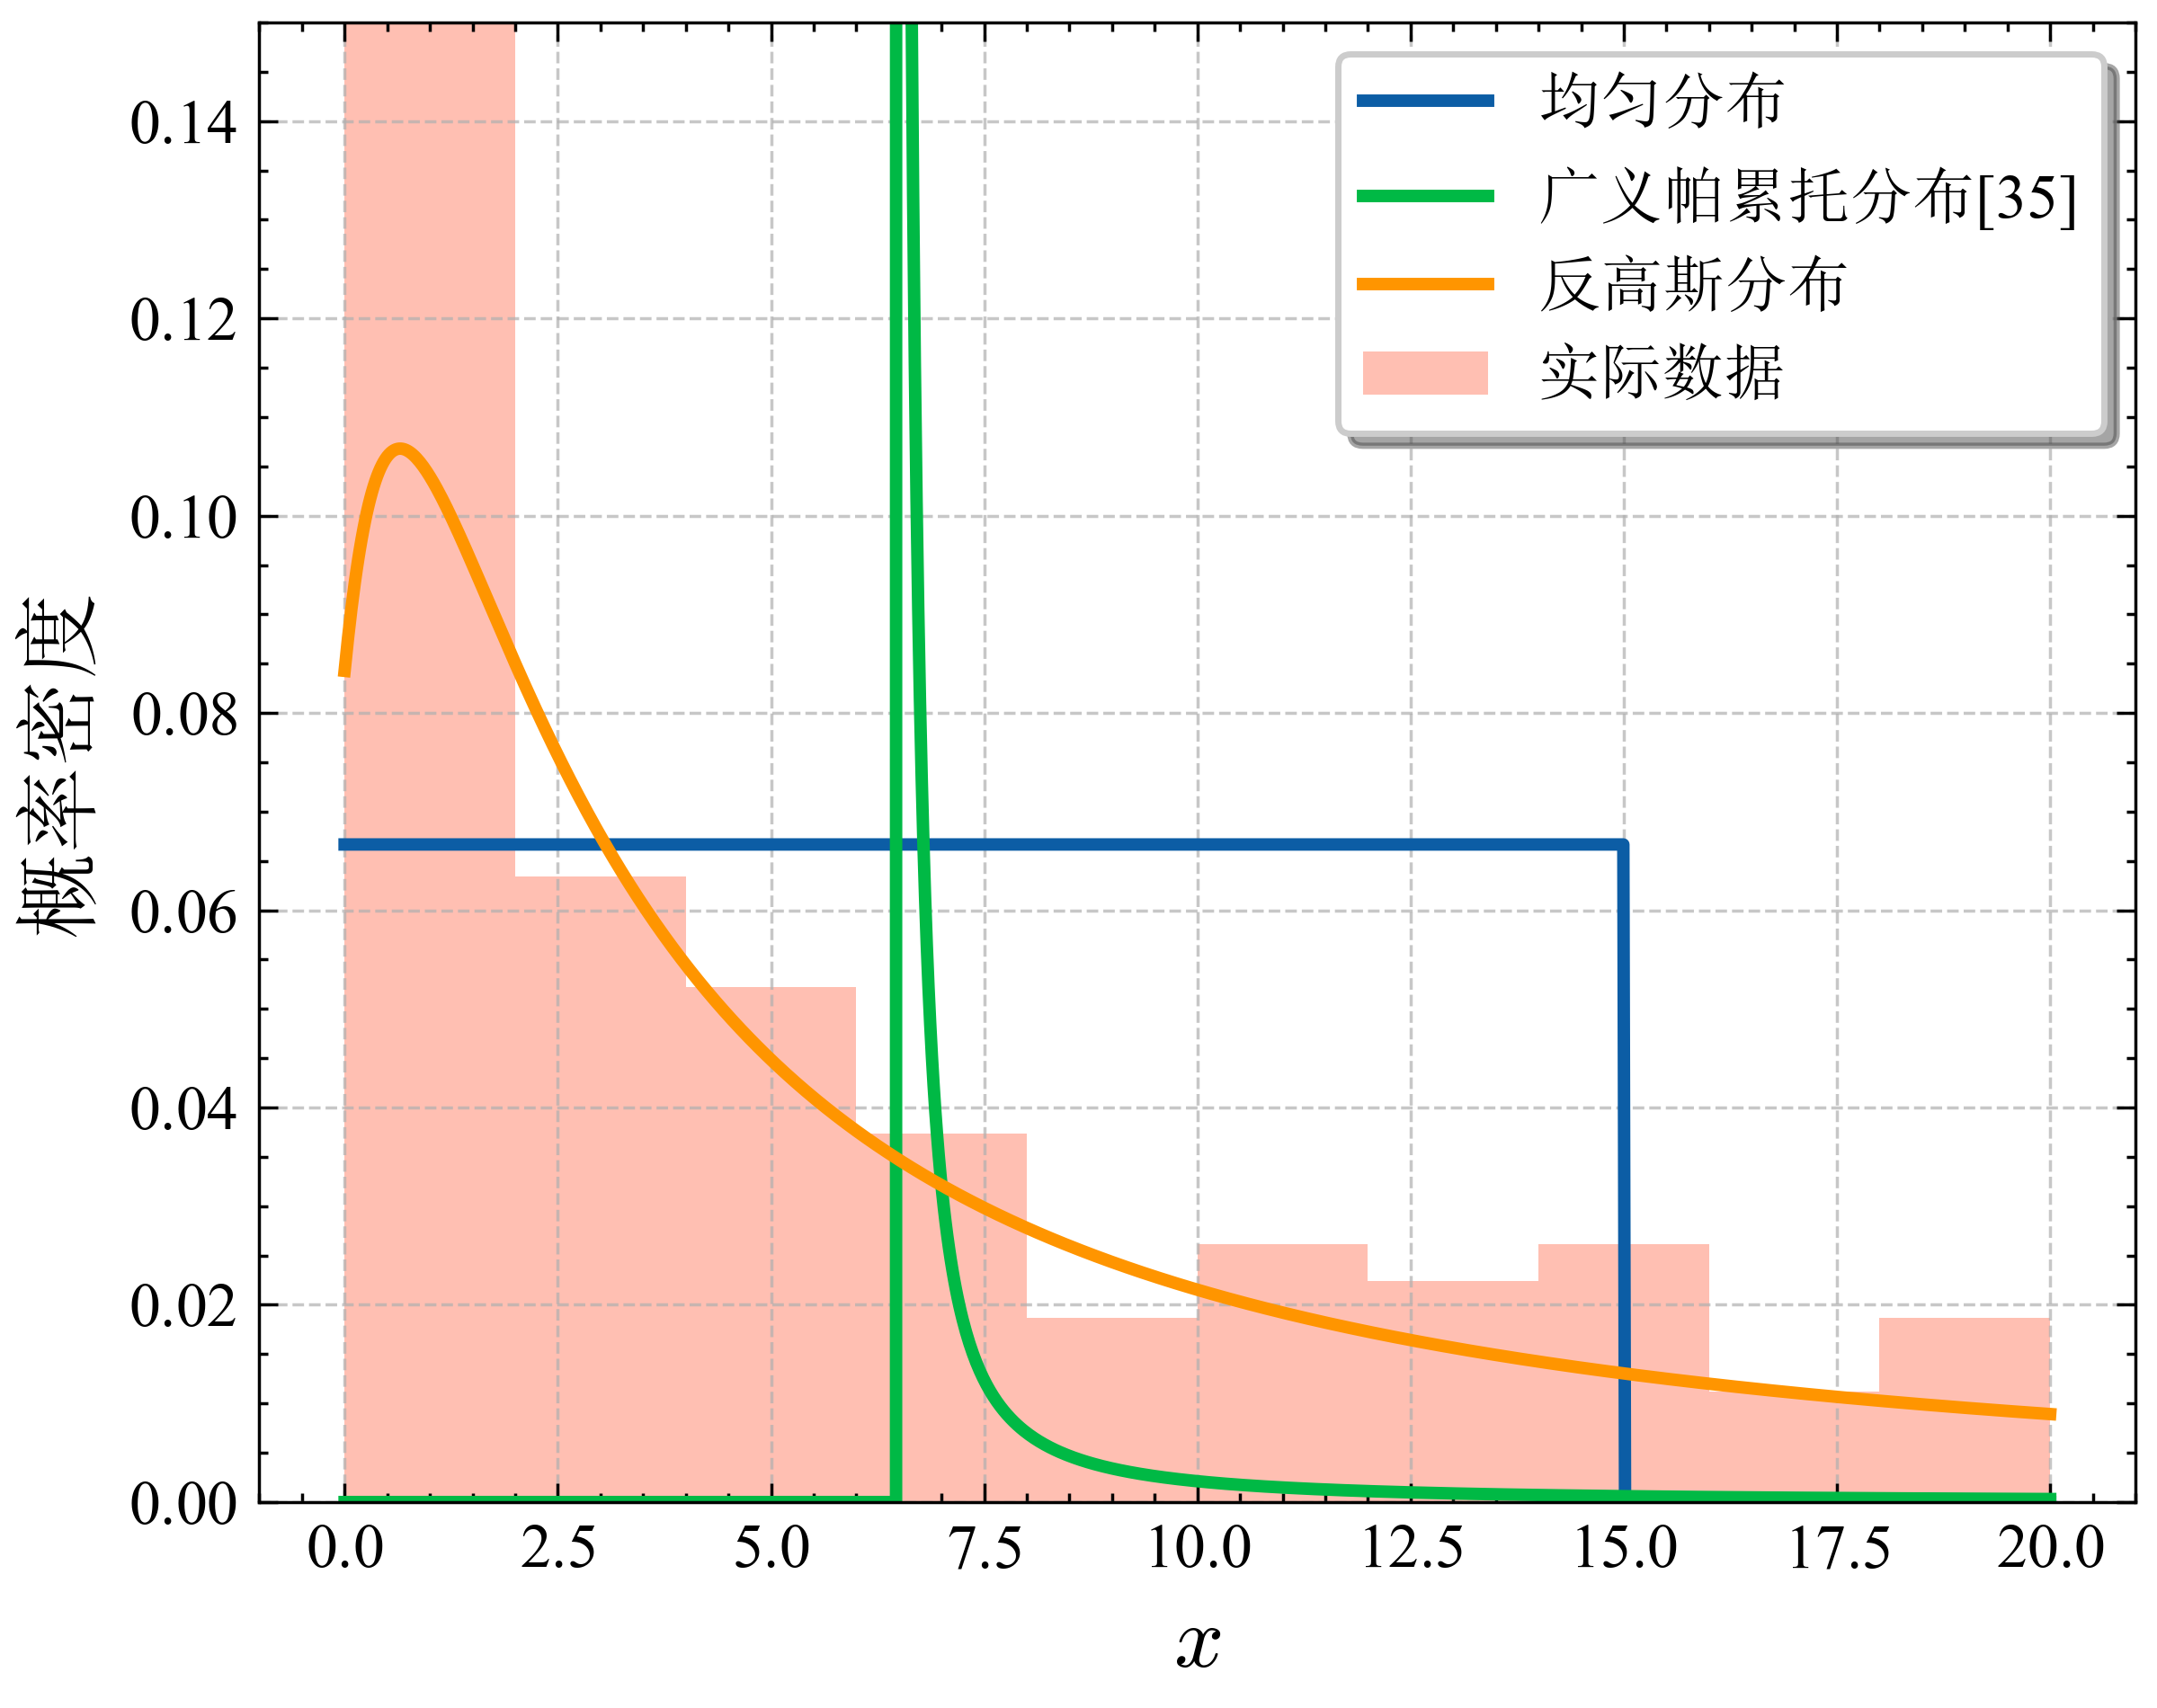
\includegraphics[width=1\linewidth]{basic_pictures/分布拟合.png}
    \caption{分布拟合结果}
    \label{fig:分布拟合}
\end{figure}
\begin{table*}[t]
\centering
\caption{不同情景下应急物资储备与利润计算结果}
\label{tab:simulation_results}
\small
\begin{tabular}{llrrrrr}
\toprule
\multicolumn{1}{c}{\textbf{情景}} & \multicolumn{1}{c}{\textbf{分布类型}} & \multicolumn{1}{c}{\textbf{$Q^*$}} & \multicolumn{1}{c}{\textbf{$q^*$}} & \multicolumn{1}{c}{\textbf{$p^*$}} & \multicolumn{1}{c}{\textbf{政府最大利润}} & \multicolumn{1}{c}{\textbf{企业最大利润}} \\
\midrule
\multirow{2}{*}{基准模型} & 均匀分布 & 5.0000 & 1.5430 & 0.3125 & -3113.7329 & 210.2559 \\
 & 反高斯分布 & 2.3420 & 0.8539 & 0.3125 & -1710.5542 & 184.1534 \\
\midrule
\multirow{2}{*}{不考虑捐赠} & 均匀分布 & 5.0000 & 2.0312 & 0.0000 & -3197.6563 & 288.7940 \\
 & 反高斯分布 & 2.3420 & 1.3519 & 0.0000 & -1767.4206 & 238.1472 \\
\midrule
\multirow{2}{*}{不考虑企业代储} & 均匀分布 & 6.4107 & 0.0000 & 0.3125 & -3115.9096 & 157.0595 \\
 & 反高斯分布 & 3.1076 & 0.0000 & 0.3125 & -1771.2785 & 164.4732 \\
\midrule
\multirow{2}{*}{\begin{tabular}[c]{@{}l@{}}不考虑企业\\代储和企业生产\end{tabular}} & 均匀分布 & 7.5000 & 0.0000 & 0.3125 & -3129.7526 & 109.9505 \\
 & 反高斯分布 & 39.7200 & 0.0000 & 0.3125 & -6123.9239 & 139.6021 \\
\bottomrule
\end{tabular}
\end{table*}
经过拟合可以发现反高斯分布的SSE最小,因此采用其对本文使用的数据集进行拟合。本算例采用的拟合概率密度函数 $f(x)$ 具体形式如下:
\begin{align}
\label{eq:pdf_demand}
f(x) = \sqrt{\frac{4.87}{2\pi (x + 0.97)^3}} \nonumber 
     \quad \times e^{\left[ -\frac{4.87 \left((x + 0.97) - 40.69\right)^2}{2(40.69)^2 (x + 0.97)} \right]}
\end{align}
其中,$x \ge 0$ 表示应急物资的需求量(单位:件)。
该概率密度函数 $f(x)$ 将被用于计算政府和企业在不同物资需求情景下的期望收益。相应的累积分布函数 $F(x) = \int_0^x f(t) dt$ 由于其解析表达式复杂,将在后续的数值计算中通过数值积分方法获得。考虑到复杂的无穷上限积分可能遇到不收敛的问题,因此本文将累积概率值为0.7处对应的物资需求量作为最大物资需求量,即积分上限$U$。

拟合结果如图\ref{fig:分布拟合}所示,该图表展示了实际数据的概率密度分布,并与三种理论概率分布模型——均匀分布(大多数文献,如\cite{LIY2023,zhengh2023,XTGL202004012}使用的)、广义帕累托分布(\cite{Li2022Stackelberg}使用的)以及反高斯分布(我们采用的)——进行了拟合比较。纵轴代表相应的概率密度。实际数据通过浅色条形柱状图(直方图)的形式呈现,显示出一种右偏的分布特征,在 $x$ 较小的区间内具有较高的概率密度,随后概率密度迅速下降。均匀分布(蓝色实线)在 $x$ 取0至约15的区间内呈现为一个恒定的概率密度值,然后骤降为零,这与实际数据的分布形态差异显著。广义帕累托分布[35](绿色实线)从约 $x=6.5$ 处开始急剧下降,未能捕捉到数据在较小 $x$ 值处的高密度区域。相比之下,反高斯分布(橙色曲线)从 $x=0$ 处开始,概率密度迅速上升至 $x$ 约$1.5$处的峰值,随后平滑下降,其整体形态与实际数据的直方图轮廓展现出较好的一致性,尤其是在峰值位置和尾部衰减趋势上。

根据图示结果可以明确,反高斯分布在描述所示实际数据的概率分布特征方面,显著优于均匀分布和广义帕累托分布。均匀分布过于简化,无法体现数据分布的峰度和偏斜特征。广义帕累托分布在本例中未能有效拟合数据的主要集中区域,其适用性较差。反高斯分布的概率密度曲线则较好地捕捉了实际数据从低位快速上升至峰值,再逐渐衰减的整体趋势,表明反高斯分布是对该组实际数据更为合适的理论分布模型。更适合后续的决策过程。

\subsection{案例计算结果与敏感性分析}
本节基于前述算例设置与构建的应急物资需求概率分布模型,利用SLSQP算法求解得到政企联合储备模型在基准参数下的最优决策,并进一步通过敏感性分析探讨关键参数变化对最优储备量、企业捐赠量及企业生产能力储备的影响。分析将分别在均匀分布和基于历史数据拟合的反高斯分布假设下进行,以揭示不同需求特征对储备策略的差异化影响。图\ref{fig:sensitivity_alpha}至图\ref{fig:sensitivity_v}展示了各参数的敏感性分析结果,图\ref{fig:structure_comparison}对比了两种分布下的最优储备结构。

\begin{figure}[H]
    \centering
    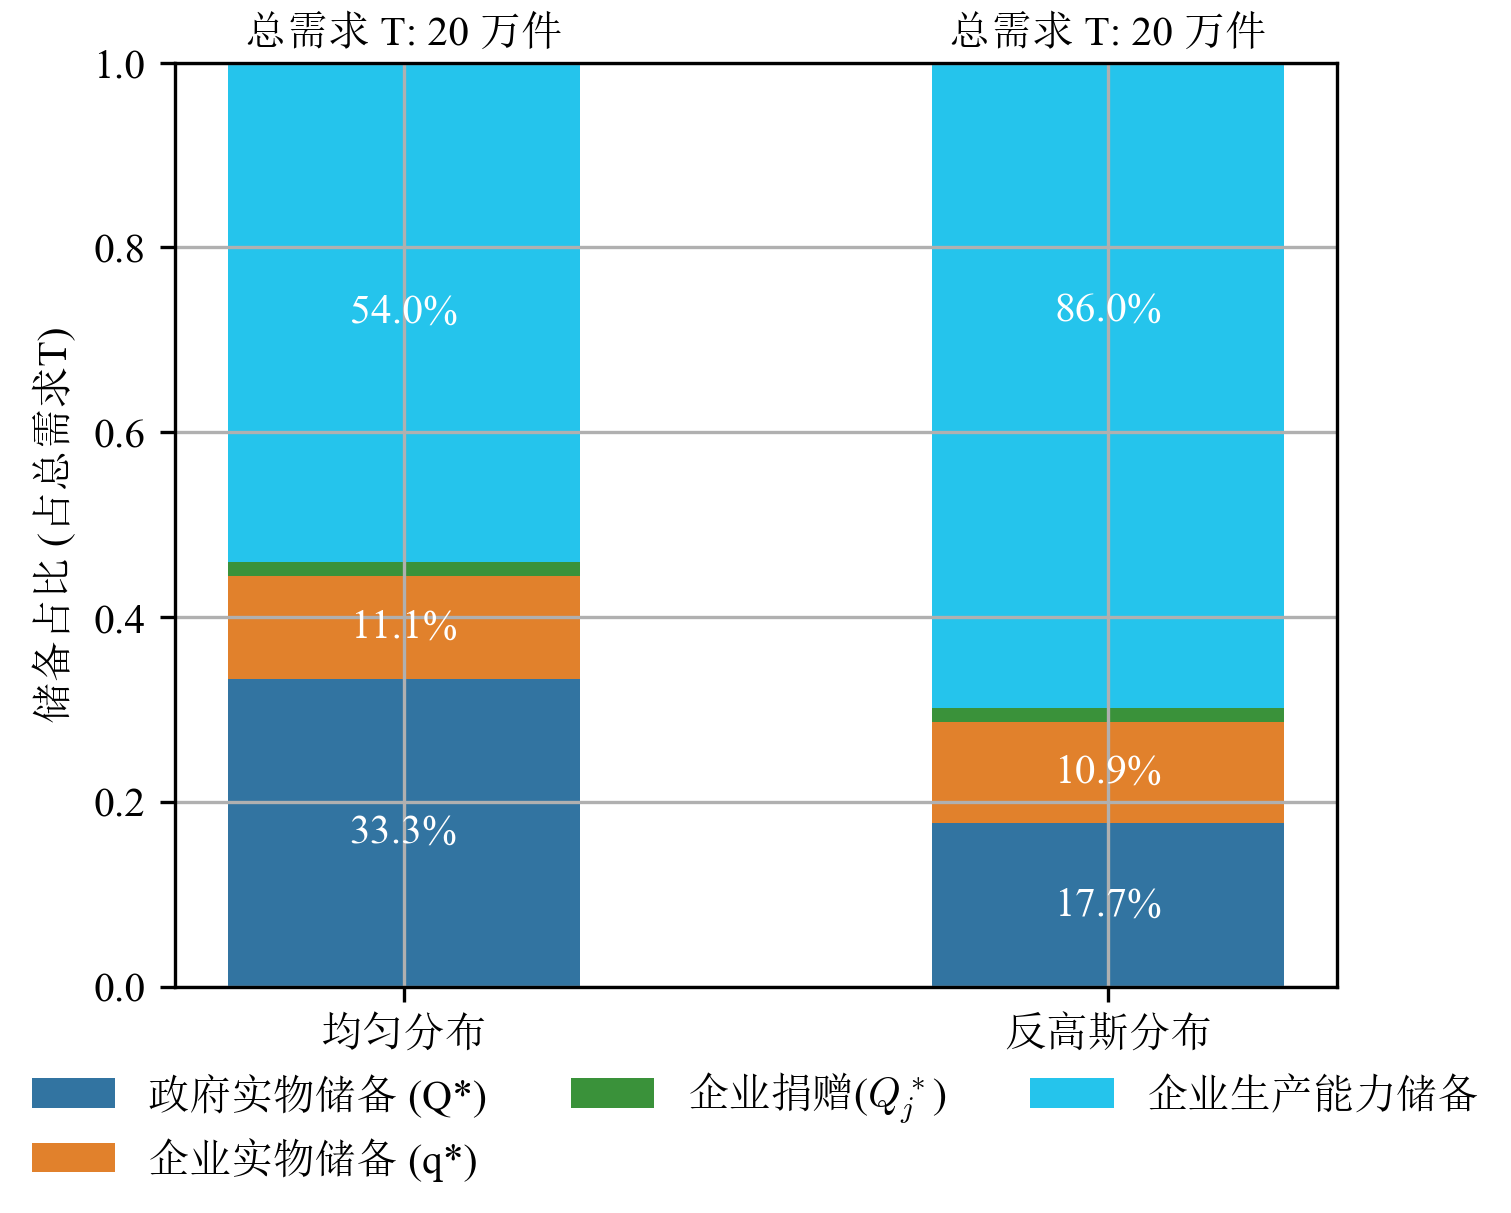
\includegraphics[width=\linewidth]{basic_pictures/储备结构对比.png}
    \caption{储备结构对比}
    \label{fig:structure_comparison}
\end{figure}

\subsubsection{不同需求分布下的最优储备结构对比}
图\ref{fig:structure_comparison}直观地对比了在总需求上限设定为15万件的条件下,均匀分布与反高斯分布假设下的最优应急物资储备结构。可以发现在均匀分布下,政府实物储备 ($Q^*$) 占比约33.3\%,企业实物储备 ($q^*$) 占比约10.3\%,企业捐赠/生产储备 ($Q_j^*$) 占比较小,而约54.3\%的需求依赖灾后的企业生产能力来满足。然而,在更贴近现实灾害需求特征的反高斯分布下,储备结构发生了变化:政府实物储备 ($Q^*$) 占比降至约15.6\%,企业实物储备 ($q^*$) 占比降至约5.7\%。这一巨大差异凸显了反高斯分布的长尾特性对储备策略的深刻影响。面对这种高度的不确定性和潜在的极端需求,预置大量实物储备的经济成本过高。因此,模型倾向于依赖更为灵活和成本效益可能更高的灾后企业生产能力。在反高斯分布下,政府和企业的实物储备更多地扮演了“首轮响应”和“争取时间”的角色,为启动更大规模的应急生产和社会动员提供缓冲。

表格\ref{tab:simulation_results}呈现了在不同预设情景及需求分布类型条件下,应急物资的最优政府储备量($Q^*$)、最优企业储备量($q^*$)、某一关键决策变量($p^*$),以及由此产生的政府与企业各自的最大利润。数据清晰地表明,多主体协同储备机制相较于单一主体储备或协同机制不完整的模式,在资源配置效率和经济效益方面展现出显著优势。

这些数值实验结果揭示了以下关键启示:首先,企业在应急物资储备体系中的参与,无论是通过协议实物代储还是产能储备,均能有效分担政府的储备压力,优化整体储备结构。例如,对比基准模型与“不考虑企业代储”及“不考虑企业代储和企业生产”情景,后两者中的政府储备量$Q^*$均显著上升,同时政府的财政支出也随之增加,尤其是在完全剥离企业参与后,政府成本急剧攀升。其次,合理的协同契约与激励机制是引导企业积极参与并发挥其效能的核心。当取消某些协同环节时,不仅影响了最优储备量,也显著改变了各方的利润水平。再者,应急物资需求的特征对最优储备策略的制定具有决定性影响,不同分布类型下的最优储备量与利润水平均存在差异。综上所述,构建一个包含政府引导、企业积极参与并辅以有效激励的多主体协同储备体系,是提升应急物资保障能力、降低社会总成本的关键路径。
\subsubsection{敏感性分析}
在应急物资多主体协同储备的Stackelberg博弈模型中,参数敏感性分析是理解储备决策机制的关键。通过对关键参数的变化进行模拟,可以揭示政府和企业储备策略的动态调整规律,为构建高效的协同储备契约提供理论依据。
\begin{figure}[H]
\centering
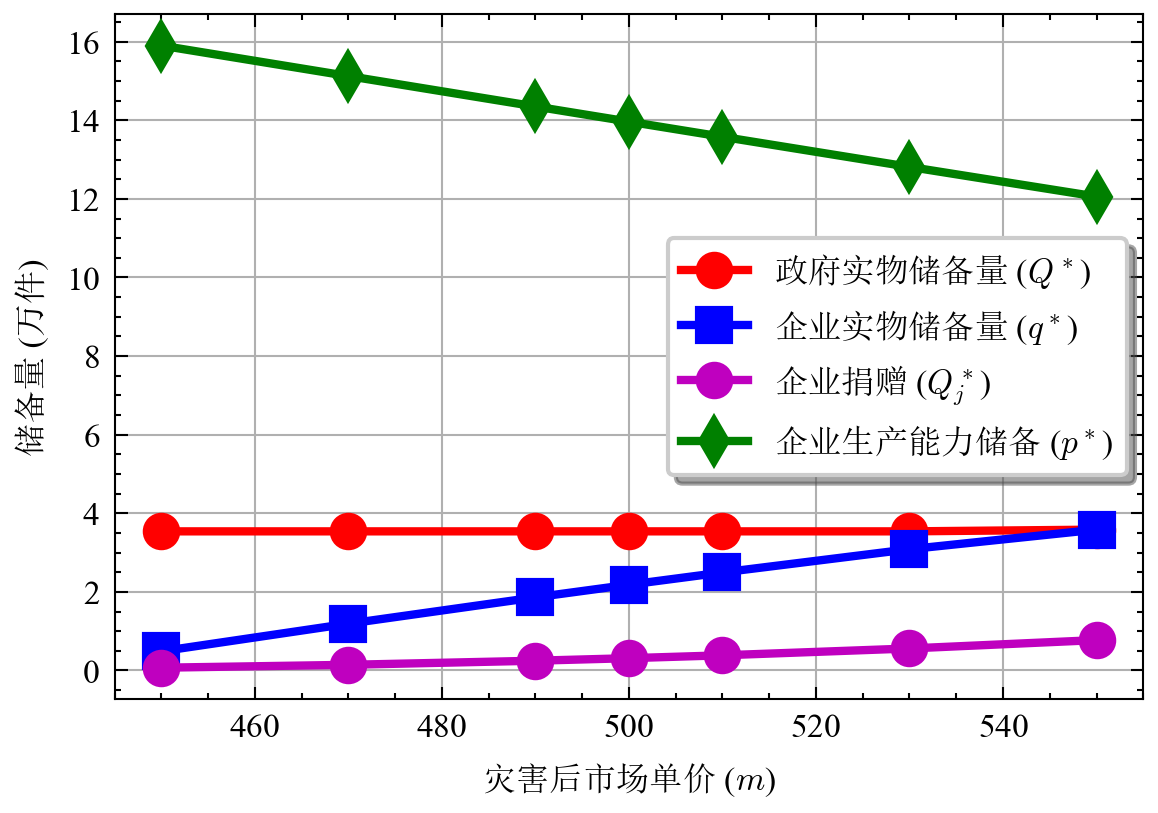
\includegraphics[width=\linewidth]{basic_pictures/sensitivity_m.png}
\caption{灾害后市场单价对储备决策的影响}
\label{fig:sensitivity_m}
\end{figure}
如图\ref{fig:sensitivity_m}所示,灾害后市场单价$(m)$的增加对各方储备决策产生显著影响。随着$m$从450元增至550元,政府实物储备量$(Q^*)$保持相对稳定,而企业实物储备量$(q^*)$和企业捐赠量$(Q_j^*)$均呈现上升趋势,企业生产能力储备$(p^*)$则呈现下降趋势。这表明灾后市场价格的提高使企业更倾向于增加实物储备和捐赠,同时减少生产能力储备投入,因为灾后高价使前期储备更具经济价值。
\begin{figure}[H]
\centering
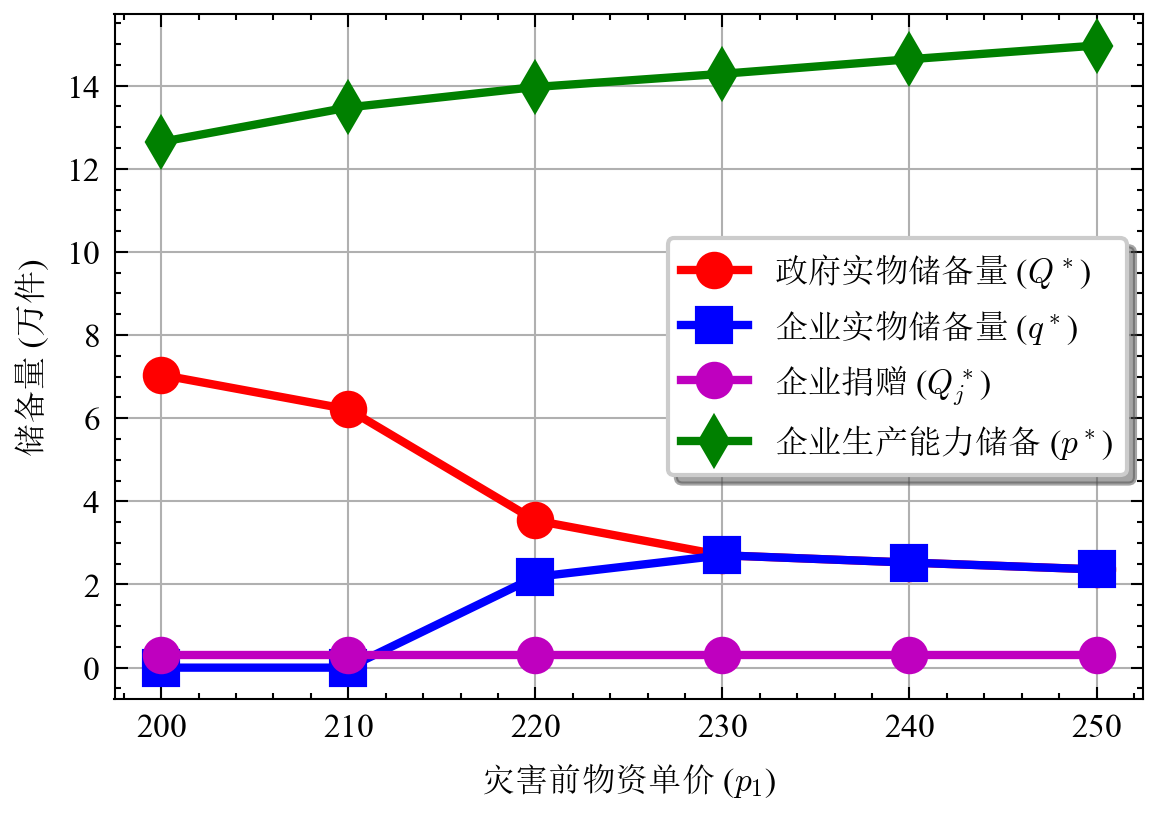
\includegraphics[width=\linewidth]{basic_pictures/sensitivity_p1.png}
\caption{灾害前物资单价对储备决策的影响}
\label{fig:sensitivity_p1}
\end{figure}
图\ref{fig:sensitivity_p1}展示了灾害前物资单价$(p_1)$对储备决策的影响。当$p_1$从200元增至250元时,政府实物储备量$(Q^*)$显著下降,而企业实物储备量$(q^*)$先增后趋于稳定。这一现象表明,灾前物资价格上涨导致政府储备成本增加,促使政府减少自身储备并将部分储备责任转移给企业。企业捐赠量$(Q_j^*)$对$p_1$变化不敏感,而企业生产能力储备$(p^*)$随$p_1$增加而增加,表明企业倾向于通过增加生产能力储备来应对高价物资储备的挑战。
\begin{figure}[H]
\centering
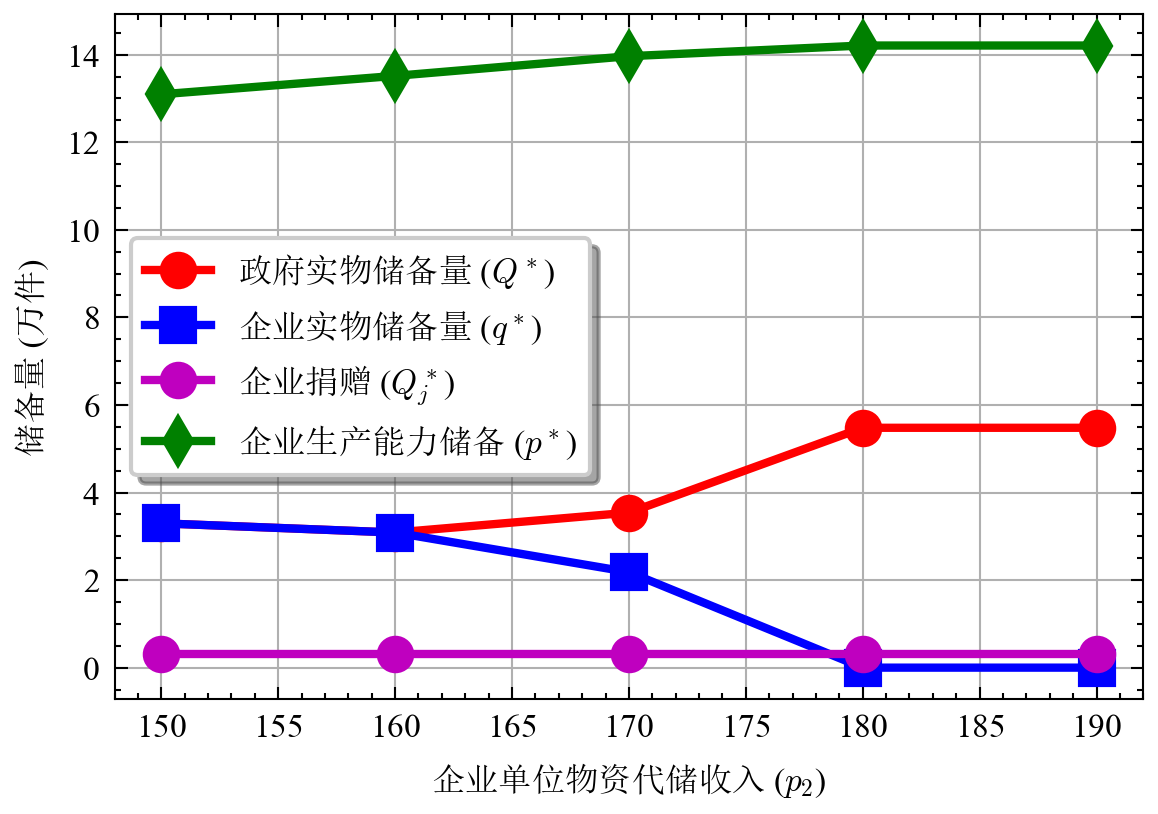
\includegraphics[width=\linewidth]{basic_pictures/sensitivity_p2.png}
\caption{企业单位物资代储收入对储备决策的影响}
\label{fig:sensitivity_p2}
\end{figure}
图\ref{fig:sensitivity_p2}分析了企业单位物资代储收入$(p_2)$的变化对储备决策的影响。随着$p_2$从150元增至190元,政府实物储备量$(Q^*)$呈现先平稳后显著增加的趋势,而企业实物储备量$(q^*)$则呈现下降趋势,当$p_2$达到180元后,企业实物储备量趋近于零。这表明企业代储收入的提高会促使政府增加对企业的委托储备,而企业则减少自身储备,转向为政府提供代储服务。企业捐赠量$(Q_j^*)$保持相对稳定,企业生产能力储备$(p^*)$略有增加,表明企业更倾向于通过提高生产能力来应对可能的灾害需求。
\begin{figure}[H]
\centering
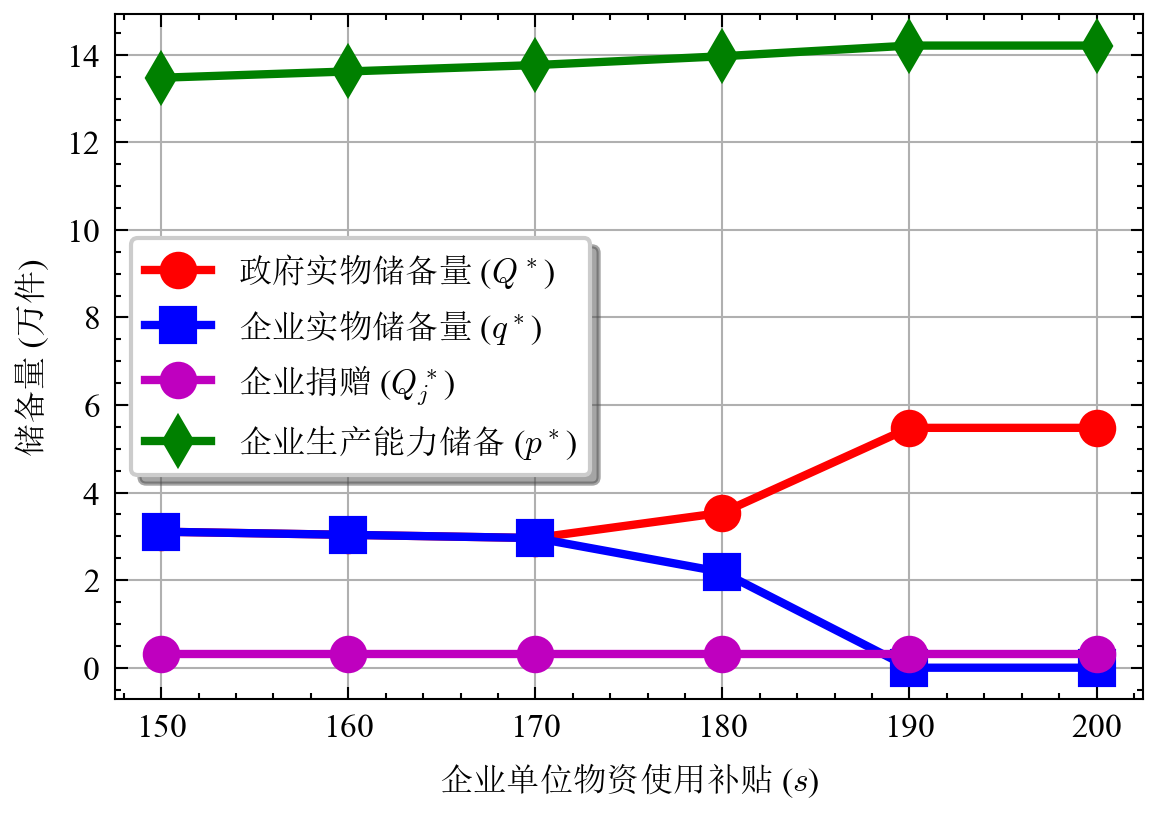
\includegraphics[width=\linewidth]{basic_pictures/sensitivity_s.png}
\caption{企业单位物资使用补贴对储备决策的影响}
\label{fig:sensitivity_s}
\end{figure}
图\ref{fig:sensitivity_s}展示了企业单位物资使用补贴$(s)$对储备决策的影响,其变化趋势与图\ref{fig:sensitivity_p2}类似。当$s$从150元增至200元时,政府实物储备量$(Q^*)$先保持稳定,后显著增加;而企业实物储备量$(q^*)$则持续下降,当$s$达到190元后接近于零。这表明政府提高物资使用补贴会促使政府增加自身储备,同时减少企业自主储备的积极性。企业捐赠量$(Q_j^*)$和企业生产能力储备$(p^*)$对$s$的变化相对不敏感,表明补贴政策主要影响实物储备结构,而非捐赠和生产能力储备决策。
\begin{figure}[H]
\centering
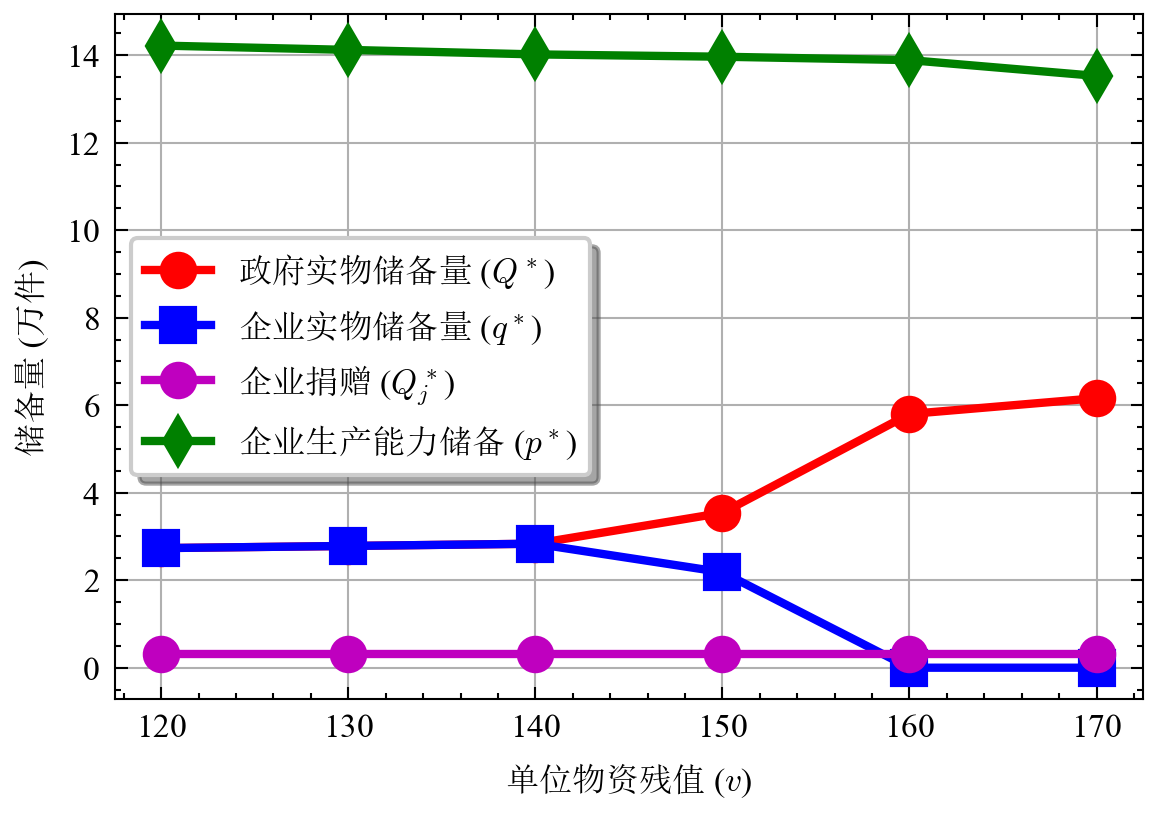
\includegraphics[width=\linewidth]{basic_pictures/sensitivity_v.png}
\caption{单位物资残值对储备决策的影响}
\label{fig:sensitivity_v}
\end{figure}
图\ref{fig:sensitivity_v}分析了单位物资残值$(v)$对储备决策的影响。随着$v$从120元增至170元,政府实物储备量$(Q^*)$显著增加,而企业实物储备量$(q^*)$先保持稳定后迅速下降至零。这表明物资残值的提高降低了政府储备的净成本,促使政府增加自身储备,而企业则减少储备投入。企业捐赠量$(Q_j^*)$对$v$的变化不敏感,企业生产能力储备$(p^*)$略有下降,表明残值的提高使企业更倾向于减少各类储备投入。
\begin{figure}[H]
\centering
\includegraphics[width=\linewidth]{basic_pictures/sensitivity_alpha.png}
\caption{灾害发生概率对储备决策的影响}
\label{fig:sensitivity_alpha}
\end{figure}
图\ref{fig:sensitivity_alpha}展示了灾害发生概率$(\alpha)$对储备决策的影响。随着$\alpha$从0.8增至1.0,政府实物储备量$(Q^*)$和企业实物储备量$(q^*)$均呈现增加趋势,表明灾害发生概率的提高促使政府和企业增加前期实物储备以应对更高的灾害风险。企业捐赠量$(Q_j^*)$对$\alpha$的变化相对不敏感,表明企业捐赠行为主要受其他因素影响。企业生产能力储备$(p^*)$随$\alpha$增加而显著下降,表明在高灾害风险情境下,企业倾向于增加实物储备而减少生产能力储备投入。
\begin{figure}[H]
\centering
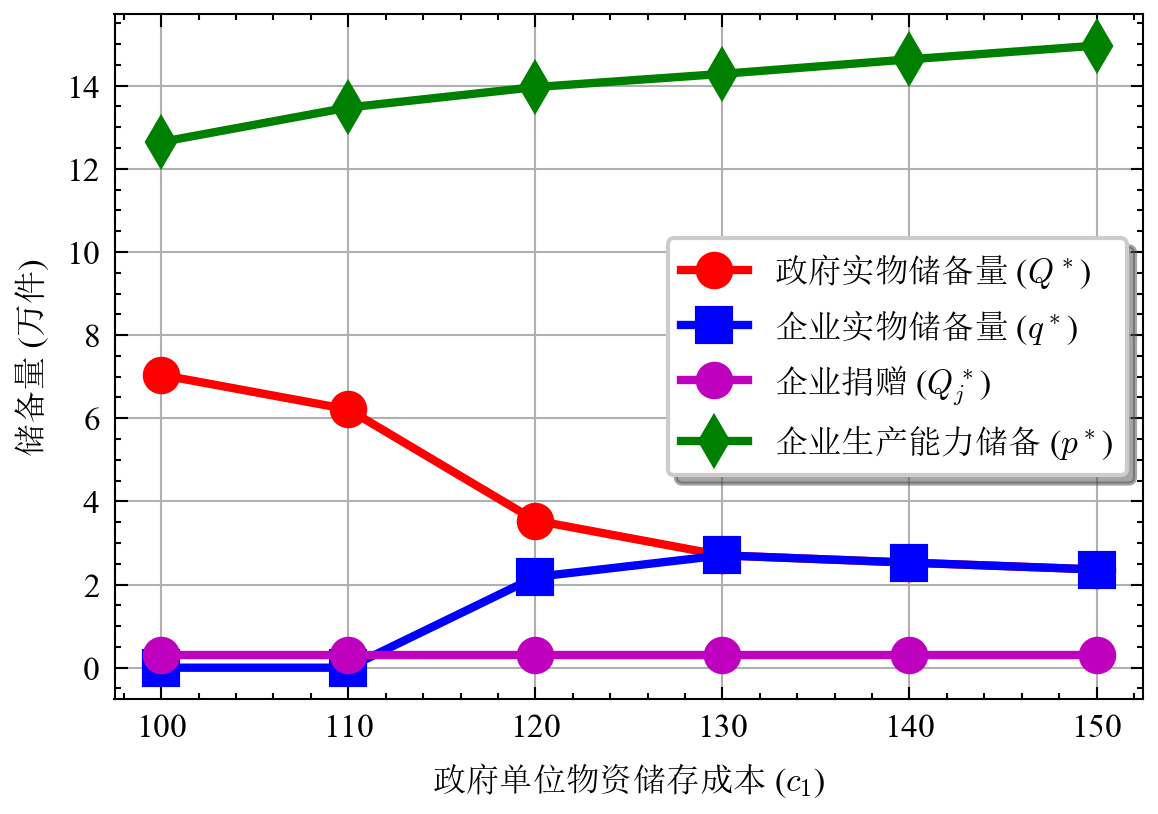
\includegraphics[width=\linewidth]{basic_pictures/sensitivity_c1.png}
\caption{政府单位物资储存成本对储备决策的影响}
\label{fig:sensitivity_c1}
\end{figure}
图\ref{fig:sensitivity_c1}分析了政府单位物资储存成本$(c_1)$对储备决策的影响。随着$c_1$从100元增至150元,政府实物储备量$(Q^*)$显著下降,而企业实物储备量$(q^*)$先为零,当$c_1$达到120元后开始增加并趋于稳定。这表明政府储存成本的增加促使政府减少自身储备并将部分储备责任转移给企业。企业捐赠量$(Q_j^*)$对$c_1$变化不敏感,企业生产能力储备$(p^*)$随$c_1$增加而增加,表明企业倾向于通过提高生产能力来应对政府储备减少带来的供应缺口。
\begin{figure}[H]
\centering
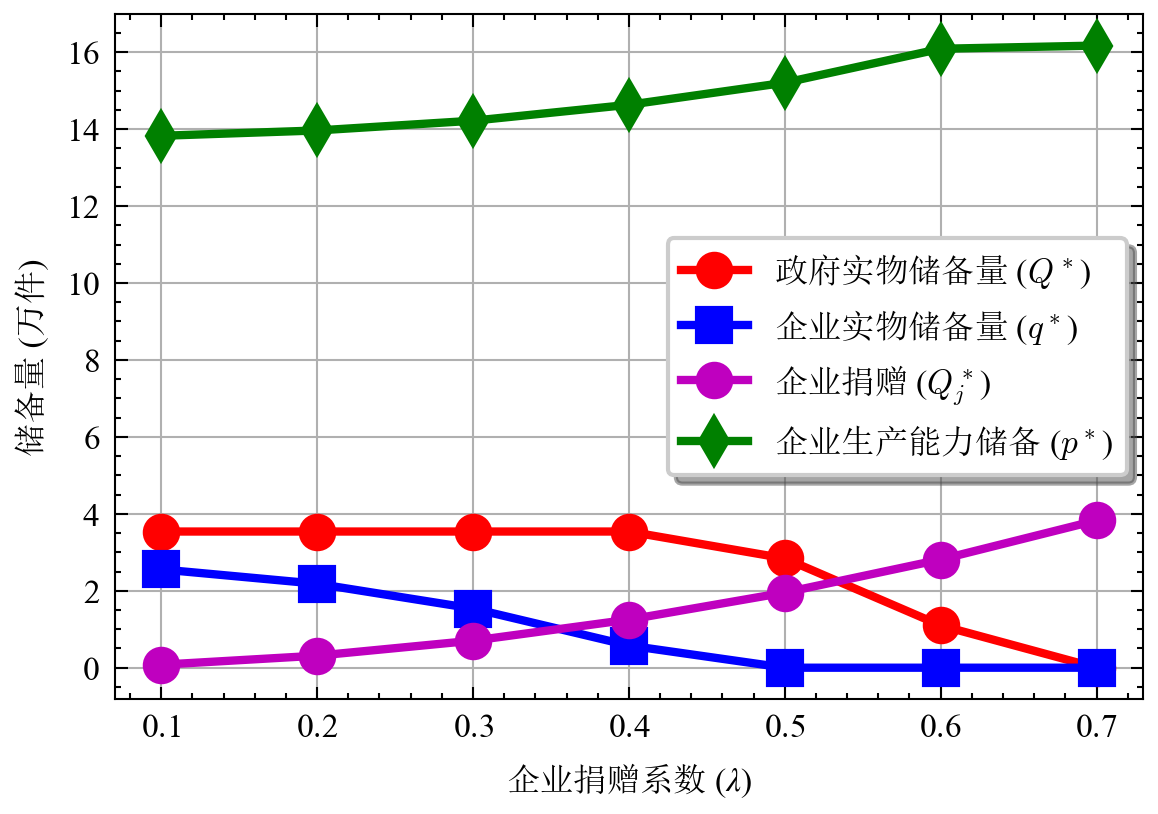
\includegraphics[width=\linewidth]{basic_pictures/sensitivity_lam.png}
\caption{企业捐赠系数对储备决策的影响}
\label{fig:sensitivity_lam}
\end{figure}
图\ref{fig:sensitivity_lam}展示了企业捐赠系数$(\lambda)$对储备决策的显著影响。随着$\lambda$从0.1增至0.7,政府实物储备量$(Q^*)$先保持稳定后显著下降,企业实物储备量$(q^*)$持续下降至零,而企业捐赠量$(Q_j^*)$则显著增加。这表明企业捐赠效益的提高促使企业增加捐赠投入,同时减少实物储备,政府也相应减少自身储备。企业生产能力储备$(p^*)$随$\lambda$增加而增加,表明企业倾向于通过提高生产能力和增加捐赠来优化其储备结构。
通过以上参数敏感性分析,可以发现政府和企业在应急物资储备决策中存在复杂的相互影响关系。政府储备政策的调整会直接影响企业的储备行为,而企业的储备策略变化也会反过来影响政府的决策。构建有效的协同储备契约需要综合考虑各种参数对储备决策的影响,以实现社会总福利最大化的目标。


\begin{table}[H]
\centering
\caption{SLSQP算法求解结果与文献精确解对比 (单位:万件)}
\label{tab:slsqp_vs_exact}
\small
\resizebox{\linewidth}{!}{
\begin{tabular}{clccc}
\toprule
分布类型 & 决策变量 & 文献精确解 & SLSQP数值解 & 相对误差 (\%) \\
\midrule
\multirow{2}{*}{均匀分布 (UD)} & $Q^*$ & 2082 & 2081.6188 & 0.0183 \\
& $q^*$ & 520  & 520.4230  & 0.0813 \\
\midrule
\multirow{2}{*}{广义帕累托分布 (GPD)} & $Q^*$ & 679 & 678.8855 & 0.0169 \\
& $q^*$ & 346 & 345.1098 & 0.2573 \\
\bottomrule
\multicolumn{5}{l}{\footnotesize 注:相对误差计算公式为 $|(\text{数值解} - \text{精确解}) / \text{精确解}| \times 100\%$}
\end{tabular}
}
\end{table}
\subsection{算法容差分析与有效性验证}
为验证本文采用的序列最小二乘二次规划 (SLSQP) 算法在求解所构建的Stackelberg模型时的有效性和准确性,本节选取了文献~\cite{LIY2023}中一个结构相对简化且能够得到精确解的应急物资储备模型作为参照。通过复现其算例参数,并利用本文提出的SLSQP算法进行求解,将数值解与文献给出的精确解进行对比。
文献~\cite{LIY2023}研究了政府主导下的应急物资政企协同储备问题,考虑了政府实物储备和企业实物储备,并将超出部分由企业生产能力满足。其模型在特定假设下可以推导出政府最优实物储备量 ($Q^*$) 和企业最优实物储备量 ($q^*$) 的数学表达式。在这一部分,我们的参数同~\cite{LIY2023}设置。

为了与文献模型进行对比,本文模型在采用上述参数时,将企业捐赠行为影响系数 $\lambda$ 设为0,从而使得企业捐赠量 $Q_j^*$ 理论上为0 (根据式\eqref{eq:optimal_Qj}),使模型结构与文献~\cite{LIY2023}中的“政府实物储备 + 企业实物储备 + 企业生产能力储备”三部分结构一致。在此设定下,使用SLSQP算法对本文模型进行求解,得到的政府最优实物储备量 $Q^*$ 和企业最优实物储备量 $q^*$ 结果如下:
\begin{itemize}
    \item 在均匀分布假设下:$Q^* = 2081.6188 \approx 2082$  万件,$q^* = 520.4230 \approx 520$ 万件。
    \item 在广义帕累托分布(假设其参数与文献一致)假设下:$Q^* = 678.8855 \approx 679$ 万件,$q^* = 345.1098 \approx 345$ 万件。
\end{itemize}

表\ref{tab:slsqp_vs_exact}将SLSQP算法的求解结果与文献~\cite{LIY2023}的精确解进行了比较。

从表\ref{tab:slsqp_vs_exact}的对比结果可以看出:
\begin{enumerate}
    \item SLSQP算法得到的数值解与文献中给出的精确解高度吻合。在均匀分布下,$Q^*$ 和 $q^*$ 的相对误差分别仅为 $0.0183\%$ 和 $0.0813\%$。
    \item 在广义帕累托分布下,$Q^*$ 和 $q^*$ 的相对误差也分别低至 $0.0169\%$ 和 $0.2573\%$。
    \item 这些微小的误差可以归因于多方面因素,包括SLSQP算法本身的数值收敛容差、文献中精确解可能存在的取整,但总的来说可以认为SLSQP算法在误差允许的范围内能高效地搜索到精确解。
\end{enumerate}

\section{结论}
本文围绕应急物资多主体协同储备问题,构建了一个政府与企业在应急物资储备上的Stackelberg模型。模型综合考虑了政府实物储备、企业实物储备和企业生产能力储备这三种主要储备方式,并考虑了由于企业社会责任可能产生的捐赠量,为应急物资储备策略提供了一种切实可行的规划方法。接着本文又对模型进行了深入分析,并利用序列二次规划(SLSQP)算法进行求解和数值实验,得到了以下主要结论和管理启示:
\begin{enumerate}
    \item 需求分布对最优储备结构具有显著影响。与传统的均匀分布假设相比,基于历史灾害数据拟合的反高斯分布更贴近现实需求,从而起到了优化政府的物资存储结构,降低政府开支的作用。这提示我们在进行应急物资储备规划时,应充分考虑需求分布的长尾特性,避免因简单采用均匀分布而导致资源浪费。
    \item 灾害发生概率的增加会促使政企增加前期实物储备,以提升应对能力。同时,企业捐赠意愿主要受捐赠效益系数影响,对灾害发生概率的变化相对不敏感。这表明政府在提升整体应急保障能力时,除了加强实物储备外,还应可以通过优化激励机制鼓励企业积极履行社会责任,例如通过提供更优惠的政策或提高企业声誉等方式激发企业捐赠的积极性。
    \item 政府和企业在应急物资储备上的决策相互影响。政府单位物资存储成本的增加会促使政府减少自身实物储备,并将部分储备压力转移给企业。而企业单位物资代储收入和单位物资使用补贴的增加,则会促使政府减少对企业代储的依赖,转而增加自身的实物储备。这提示政府在设计与企业合作的储备契约时,需要平衡各方利益,合理设置代储费用和使用补贴,以实现整体效益最大化。
    \item 灾后应急物资市场单价和单位物资残值的增加,会降低实物储备的净持有成本,从而促使政企增加实物储备量。这与直觉相符,也进一步验证了模型的有效性。
    \item 本文采用的序列二次规划算法在求解所构建的Stackelberg模型时表现出较高的有效性和准确性。通过与简化模型的精确解进行对比,数值结果表明SLSQP算法能够在误差允许的范围内高效地搜索到最优解。
\end{enumerate}

本研究的贡献在于构建了一个更为全面且贴近现实的政企联合应急物资储备决策模型,考虑了企业社会责任和多种储备方式的协同效应。通过对模型的分析和数值实验,为政府和企业在应急物资储备规划和契约设计上提供了理论基础和管理启示。
然而,本研究也存在一些不足之处。例如,模型假设物资需求在灾害发生时即刻发生,未考虑需求随时间动态变化的情况;模型也未深入探讨不同类型物资(如紧急医疗物资、生活必需品等)的差异以及多层级供应链结构的影响。未来的研究可以在这些方面进行拓展,构建更加复杂和贴近实际的应急物流储备模型,并进一步探索更加精巧的契约机制设计,以提升应急物资保障体系的韧性和效率。


\renewcommand*{\bibfont}{\footnotesize}

\printbibliography


\end{document}



